\documentclass[conference]{IEEEtran}
\IEEEoverridecommandlockouts
% The preceding line is only needed to identify funding in the first footnote. If that is unneeded, please comment it out.
\usepackage{cite}
\usepackage{amsmath,amssymb,amsfonts}
\usepackage{algorithmic}
\usepackage{graphicx}
\usepackage{textcomp}
\usepackage{pdfpages}
\usepackage{hyperref}
\usepackage{xcolor}
\def\BibTeX{{\rm B\kern-.05em{\sc i\kern-.025em b}\kern-.08em
    T\kern-.1667em\lower.7ex\hbox{E}\kern-.125emX}}
\begin{document}
\title{Implementación de Procesos de Gobierno de TI\\
{\footnotesize \textsuperscript}
}

\author{\IEEEauthorblockN{1\textsuperscript{st} Karian Yadosin Cascante Alvarez}
\IEEEauthorblockA{\textit{Facultad de Ingeniería} \\
\textit{Universidad Fidélitas }\\
\textit{San José, Costa Rica}\\
kcascante70653@ufide.ac.cr}\\
\and
\IEEEauthorblockN{2\textsuperscript{nd} Guillermo Jiménez Varela}
\IEEEauthorblockA{\textit{Facultad de Ingeniería} \\
\textit{Universidad Fidélitas }\\
\textit{San José, Costa Rica}\\
gjimenez30305@ufide.ac.cr}
\and
\IEEEauthorblockN{3\textsuperscript{rd} Kendall Ricardo Piedra Navarro}
\IEEEauthorblockA{\textit{Facultad de Ingeniería} \\
\textit{Universidad Fidélitas }\\
\textit{San José, Costa Rica}\\
kpiedra40332@ufide.ac.cr}
\and
\IEEEauthorblockN{4\textsuperscript{th} Josue David Serrano Bonilla}
\IEEEauthorblockA{\textit{Facultad de Ingeniería} \\
\textit{Universidad Fidélitas }\\
\textit{San José, Costa Rica}\\
jserrano20261@ufide.ac.cr}\\
\and
\IEEEauthorblockN{5\textsuperscript{th} Luis Diego Valverde Navarro}
\IEEEauthorblockA{\textit{Facultad de Ingeniería} \\
\textit{Universidad Fidélitas }\\
\textit{San José, Costa Rica}\\
lvalverde40214@ufide.ac.cr}
}

\maketitle

\begin{abstract}
This project seeks to implement a proposal that provides a possible solution to the management problems of the IT governance of the organization. In the case of study, it is exposed to a Central American company whose main objective is to create custom software in such a way that it has positioned itself in the region in a very solid way, however it has some drawbacks with the IT management and governance issue. .
\end{abstract}

\begin{IEEEkeywords}
IT Governance, COBIT5, ITIL.
\end{IEEEkeywords}

\section{Introducción}
\subsection{Descripción del proyecto}

El propósito fundamental del proyecto de consultoría de los procesos de la gobernabilidad de TI es encontrar debilidades o falencias en los procesos que impidan que el departamento de TI y se vean afectadas limitando su desarrollo y a su vez impidiendo alcanzar las metas de la entidad por lo que se analizará la factibilidad de implantación de las soluciones encontradas en el estudio realizado.

\subsection{Objetivos}
Rastrear y evidenciar debilidades en TI con el fin de desarrollar una propuesta de implementación de procesos de gestión de tecnología de información que ayude a mejorar la capacidad de resolución de tareas.


\subsection{Contexto del proyecto}
Centrosoft es una empresa que brinda soluciones de software para entidades gubernamentales y privadas por lo que contribuye importante al fortalecimiento y a la evolución tecnológica del país y de la zona además brinda trabajo a las comunidades cercanas y desarrolla relaciones con otras entidades a las cuales se les brinda la opción de crecer mediante el consumo de los servicios que proporcionan.


\section{Análisis de la situación actual.}
\hbox{}
\subsection{Procesos Actuales del Departamento}
\hbox{}
   \subsubsection{ \textbf{Gerencia de TI}}
   \hbox{}
        \begin{itemize}
        \item Administración de las bases de datos internas de control de empleados.
        \item Administra y desarrolla los sitios internos de la empresa.
        \item Compras de activos de software y hardware.
        \item Gestiona el centro de redes.
        \end{itemize}
    \hbox{}
    \subsubsection{ \textbf{Jefatura del Departamento de Innovación y Desarrollo}}
    \hbox{}
        \begin{itemize}
        \item Configurar los ambientes de desarrollo y de producción en Azure.
        \item Configuración de los equipos y del software necesario.
        \item Análisis y diseño de los módulos solicitados.
        \item Velar por el correcto cumplimiento de las funciones asignadas.
        \item Integraciones de código en la rama principal.
        \item Planificar la implantación.
        \item Ejecutar dicha implantación en el ambiente de producción.
        \item Ejecutar los scripts en la base de datos.
        \item Calendarizar los respaldos de código.
        \end{itemize}
    \hbox{}
    \subsubsection{ \textbf{Analista o Programador}}
    \hbox{}
        \begin{itemize}
        \item Análisis, diseño y la implementación de los diferentes módulos de los sistemas.
        \item Apoyo para la toma de decisiones.
        \item Realizar avances diarios en la Intranet indicando qué acciones se realizaron.
        \item Responsable en llevar el control de sus tareas en un tablero de Kanban.
        \end{itemize}
    \hbox{}
    \subsubsection{ \textbf{Encargado de Producto / Jefe de Calidad}}
    \hbox{}
        \begin{itemize}
        \item Dirigir el departamento de aseguramiento de la calidad.
        \item Encargado de producto el cual se encarga de tomar requerimientos de clientes.
        \item Planifica y calendariza junto con el jefe del departamento de desarrollo los pases a producción.
        \item Indicar al departamento de resolver las dudas del departamento de servicio al cliente.
        \item Indica al departamento de desarrollo las incidencias que se encontraron por medio de la Intranet.
        \item Revisa junto con el gestor de calidad que tiene a cargo las funcionalidades de los sistemas en el proceso de desarrollo, beta y seguimiento en producción.
        \end{itemize}
    \hbox{}
   \subsubsection{ \textbf{Gestor de calidad}}
   \hbox{}
        \begin{itemize}
        \item Revisar las funcionalidades del sistema.
        \item Reportar las incidencias que se encuentran.
        \item Velar durante los pases a producción que no existan inconsistencias en la información y cálculos.
        \end{itemize}
    \hbox{}
    \subsubsection{ \textbf{Encargado de soporte}}
    \hbox{}
        \begin{itemize}
        \item Brinda servicio de soporte a los clientes de la empresa.
        \item Informa al departamento de calidad.
        \item Programan las capacitaciones de los nuevos clientes para explicarles el sistema.
        \item Realizar la configuración del sistema correctamente.
        \end{itemize}
    \hbox{}

\subsection{Personal involucrado}
\hbox{}
    \begin{center}
        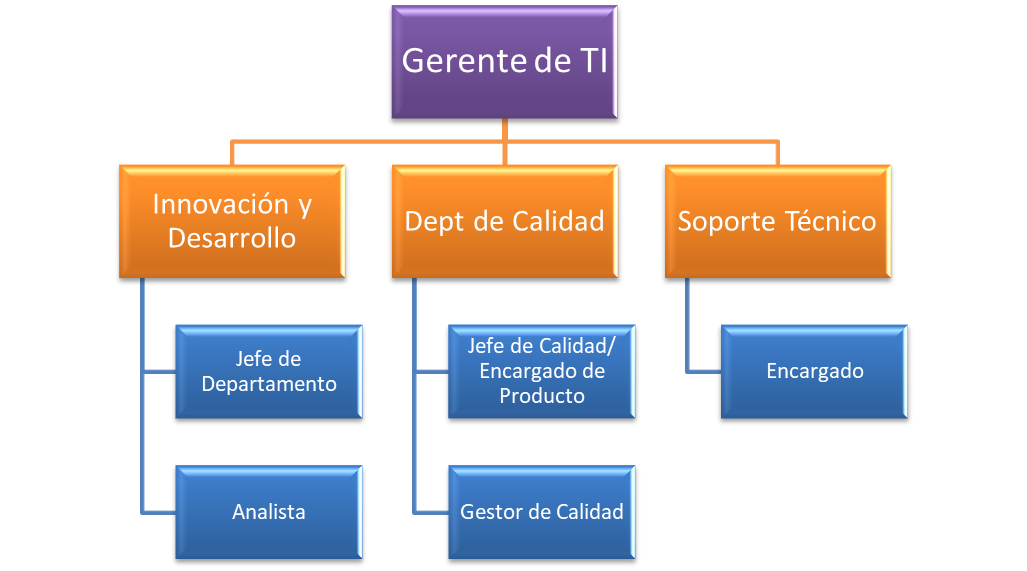
\includegraphics[width=.5\textwidth]{Imagenes/Organigrama Viejo.png}
        \textbf {Estructura organizativa del departamento de TI}
    \end{center}
\hbox{}
\subsection{Matriz de Roles y Responsabilidades}
        \begin{center}
            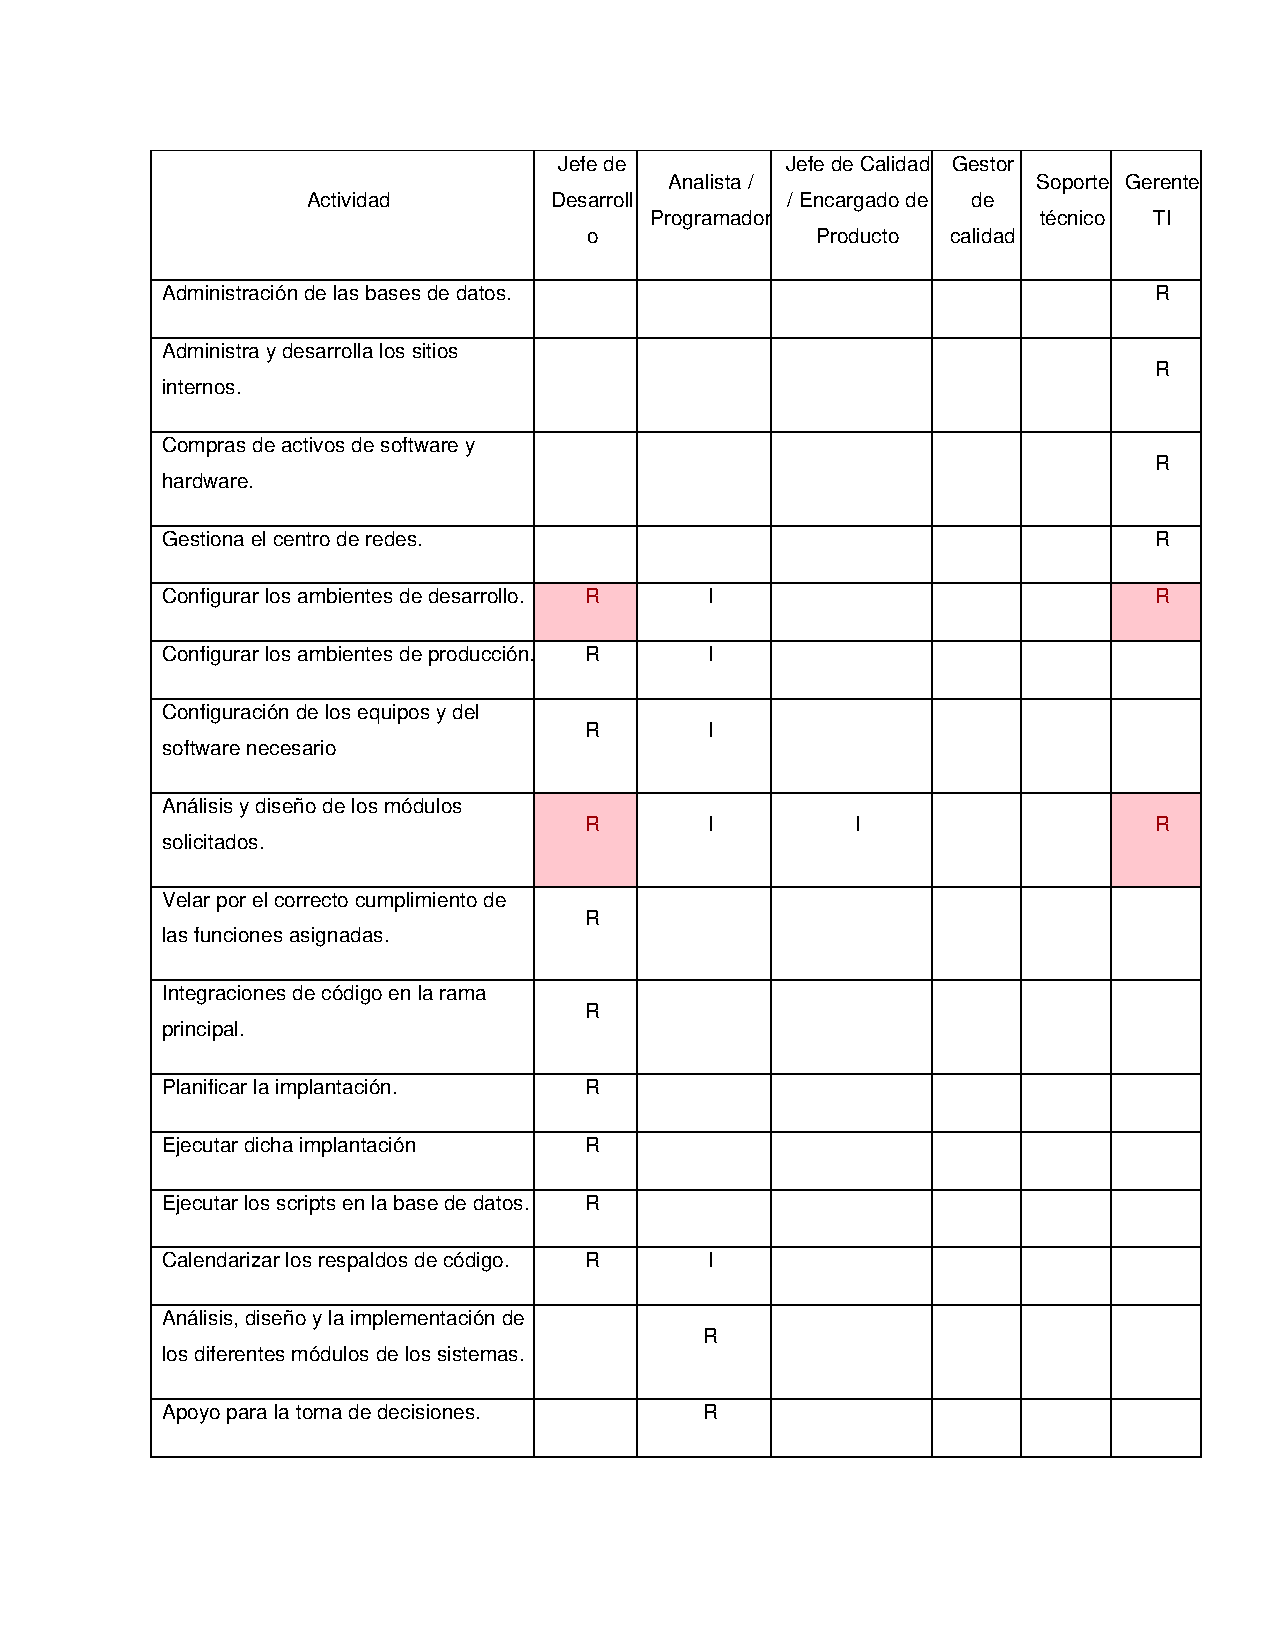
\includegraphics[width=.5\textwidth]{Documentos/Matriz RACI01.pdf}
            \textbf {Análisis de Riesgos}
        \end{center}
        
\subsection{Análisis del gobierno de TI de la empresa}
\hbox{}
    \begin{itemize}
    \item No existen control de los beneficios obtenidos de cada inversión de TI, entonces esto lleva a que la empresa desconozca si verdaderamente las inversiones realizadas fueron eficientes o no.
    \item Los recursos que tiene la empresa no tienen control, no se sabe si fueron asignados de manera correcta, o se puede estar presentando el desaprovecho de los mismos. 
    \item Los activos de la empresa no cuentan con un control de implementación y operación, por lo cual la empresa desconoce si estos están siendo utilizados para el objetivo planteado. 
    \item Algunos aspectos técnicos se encuentran mal implementados, y no existe un control sobre estos. 
    \item La empresa tampoco presenta un plan para el manejo de la gestión y control de riesgos, gestión del rendimiento o un buen manejo de sus recursos.
    \end{itemize}

\subsection{FODA}
    \begin{center}
        \textbf {Fortalezas identificadas}
        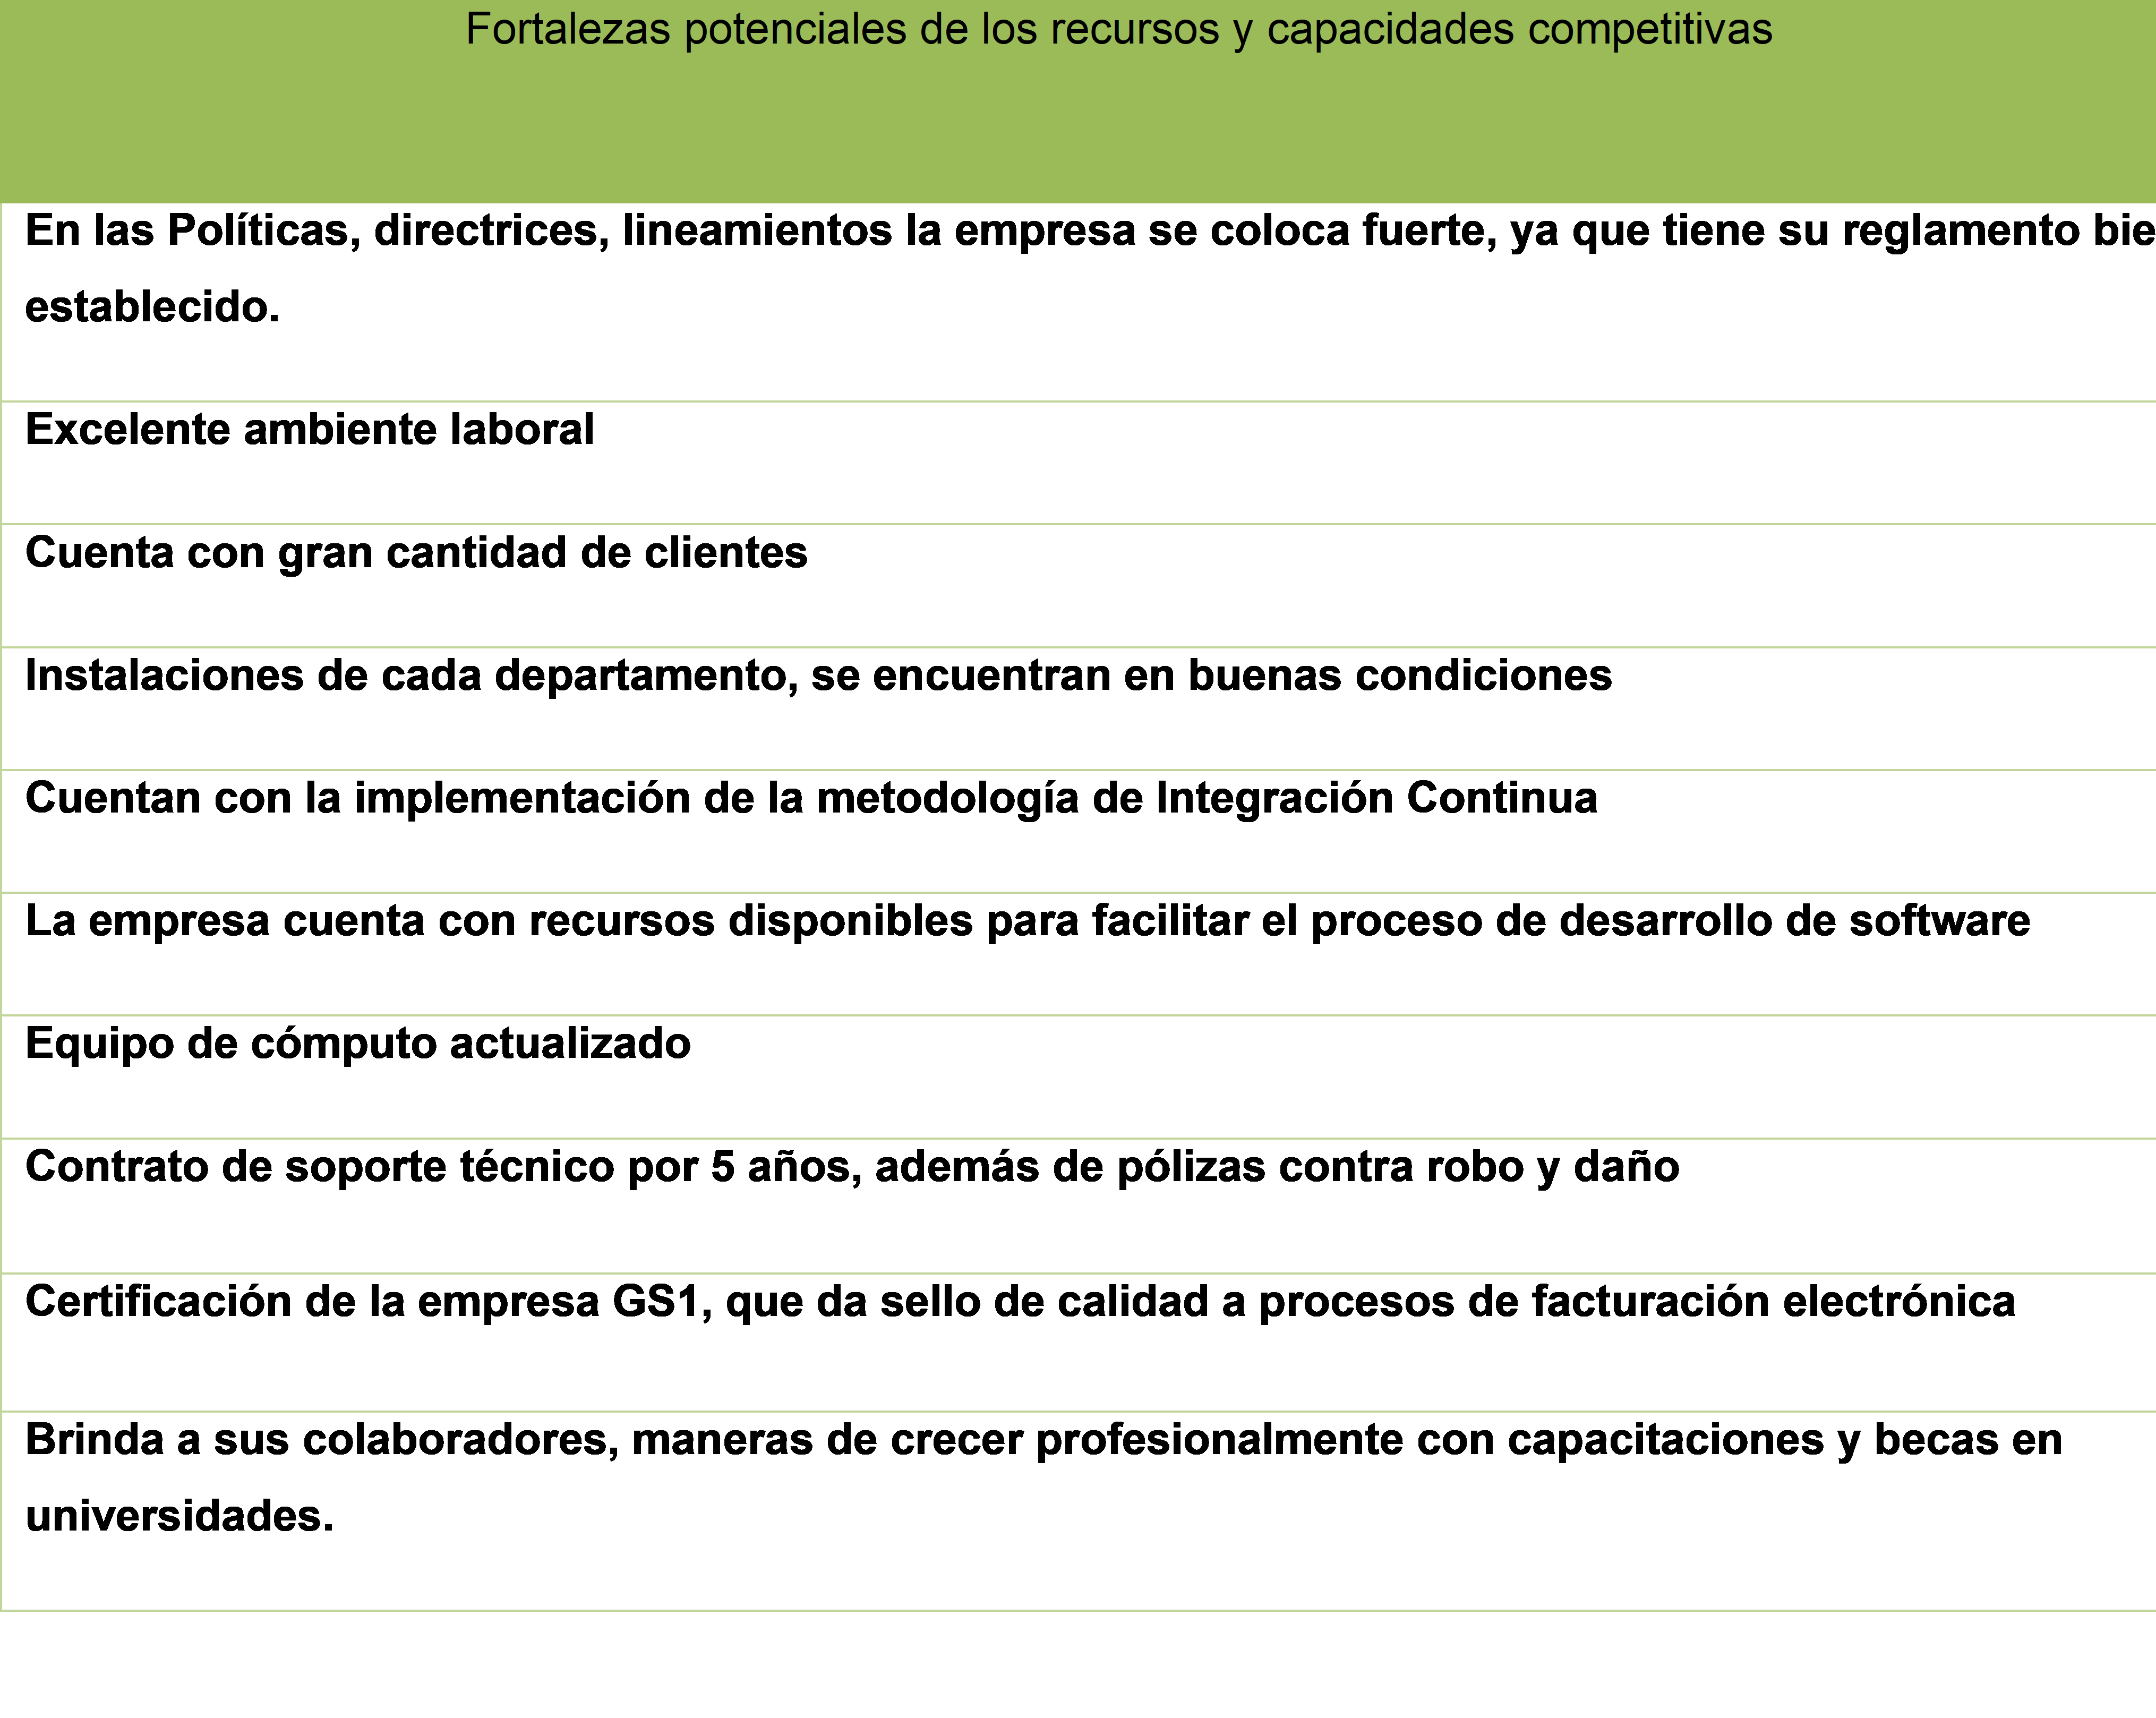
\includegraphics[width=.45\textwidth]{Imagenes/FOFA - Fortalezas.png}
        \textbf {Oportunidades identificadas}
        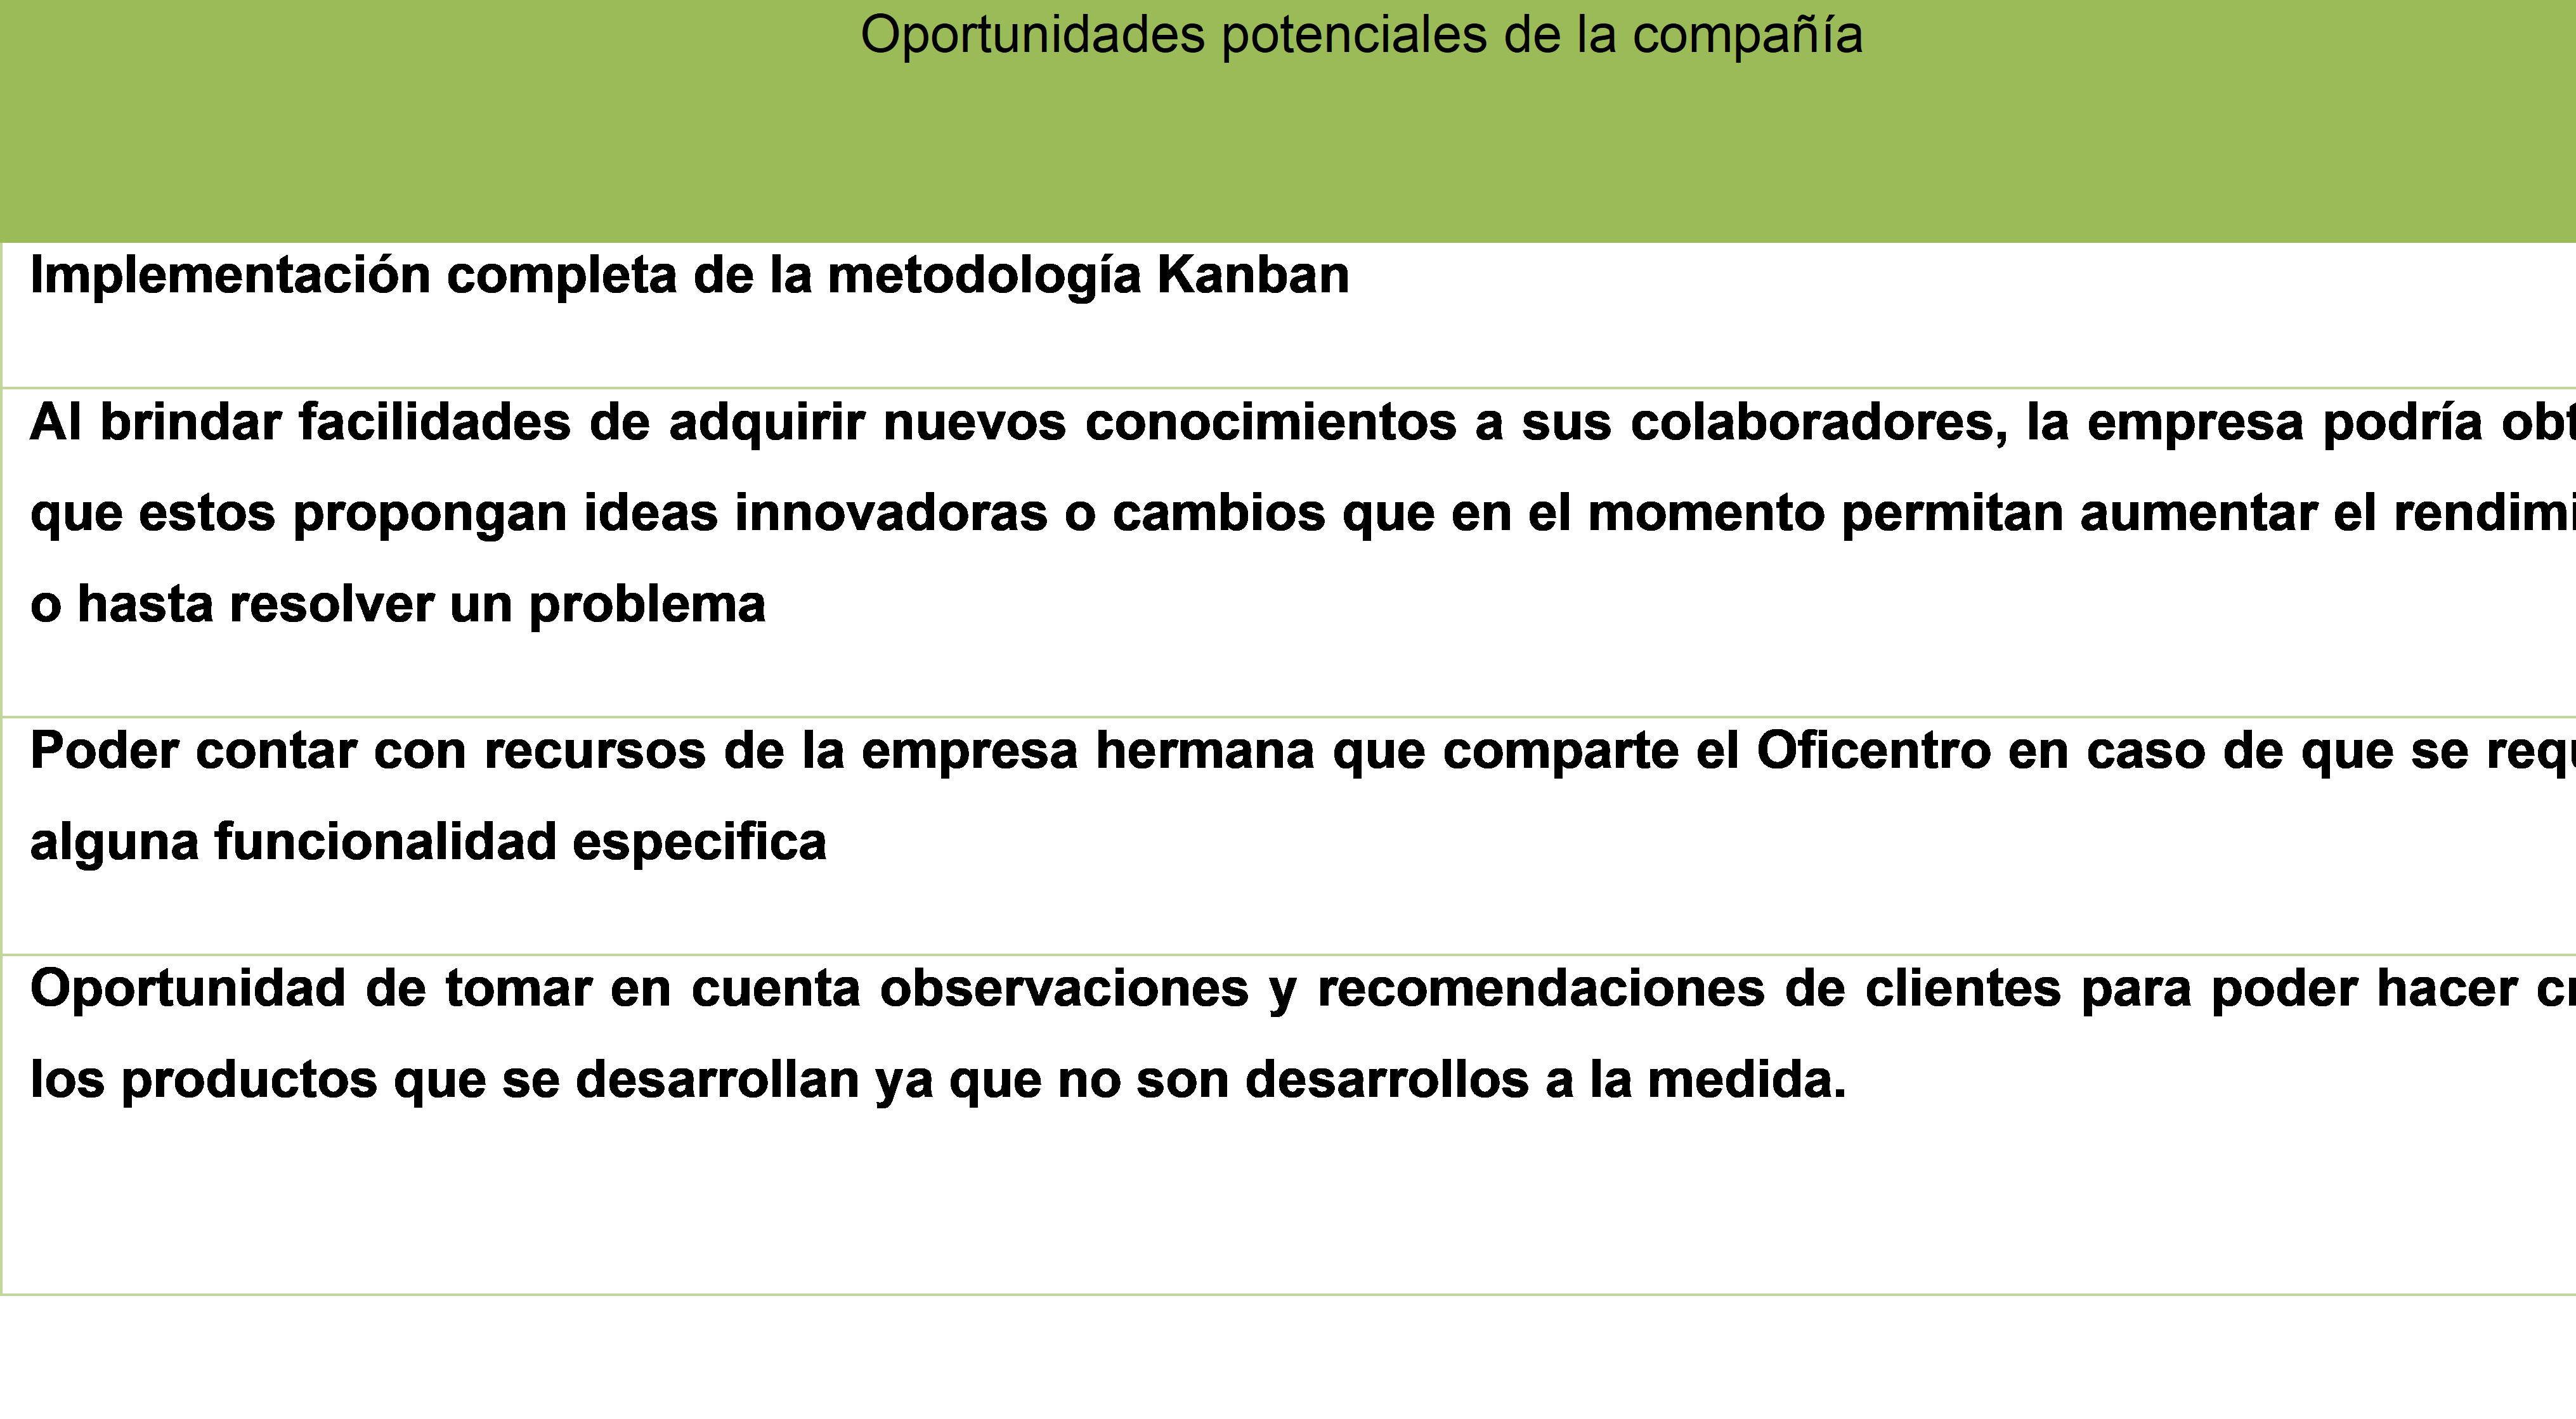
\includegraphics[width=.45\textwidth]{Imagenes/FOFA - Oportunidades.png}
        \textbf {Debilidades identificadas}
        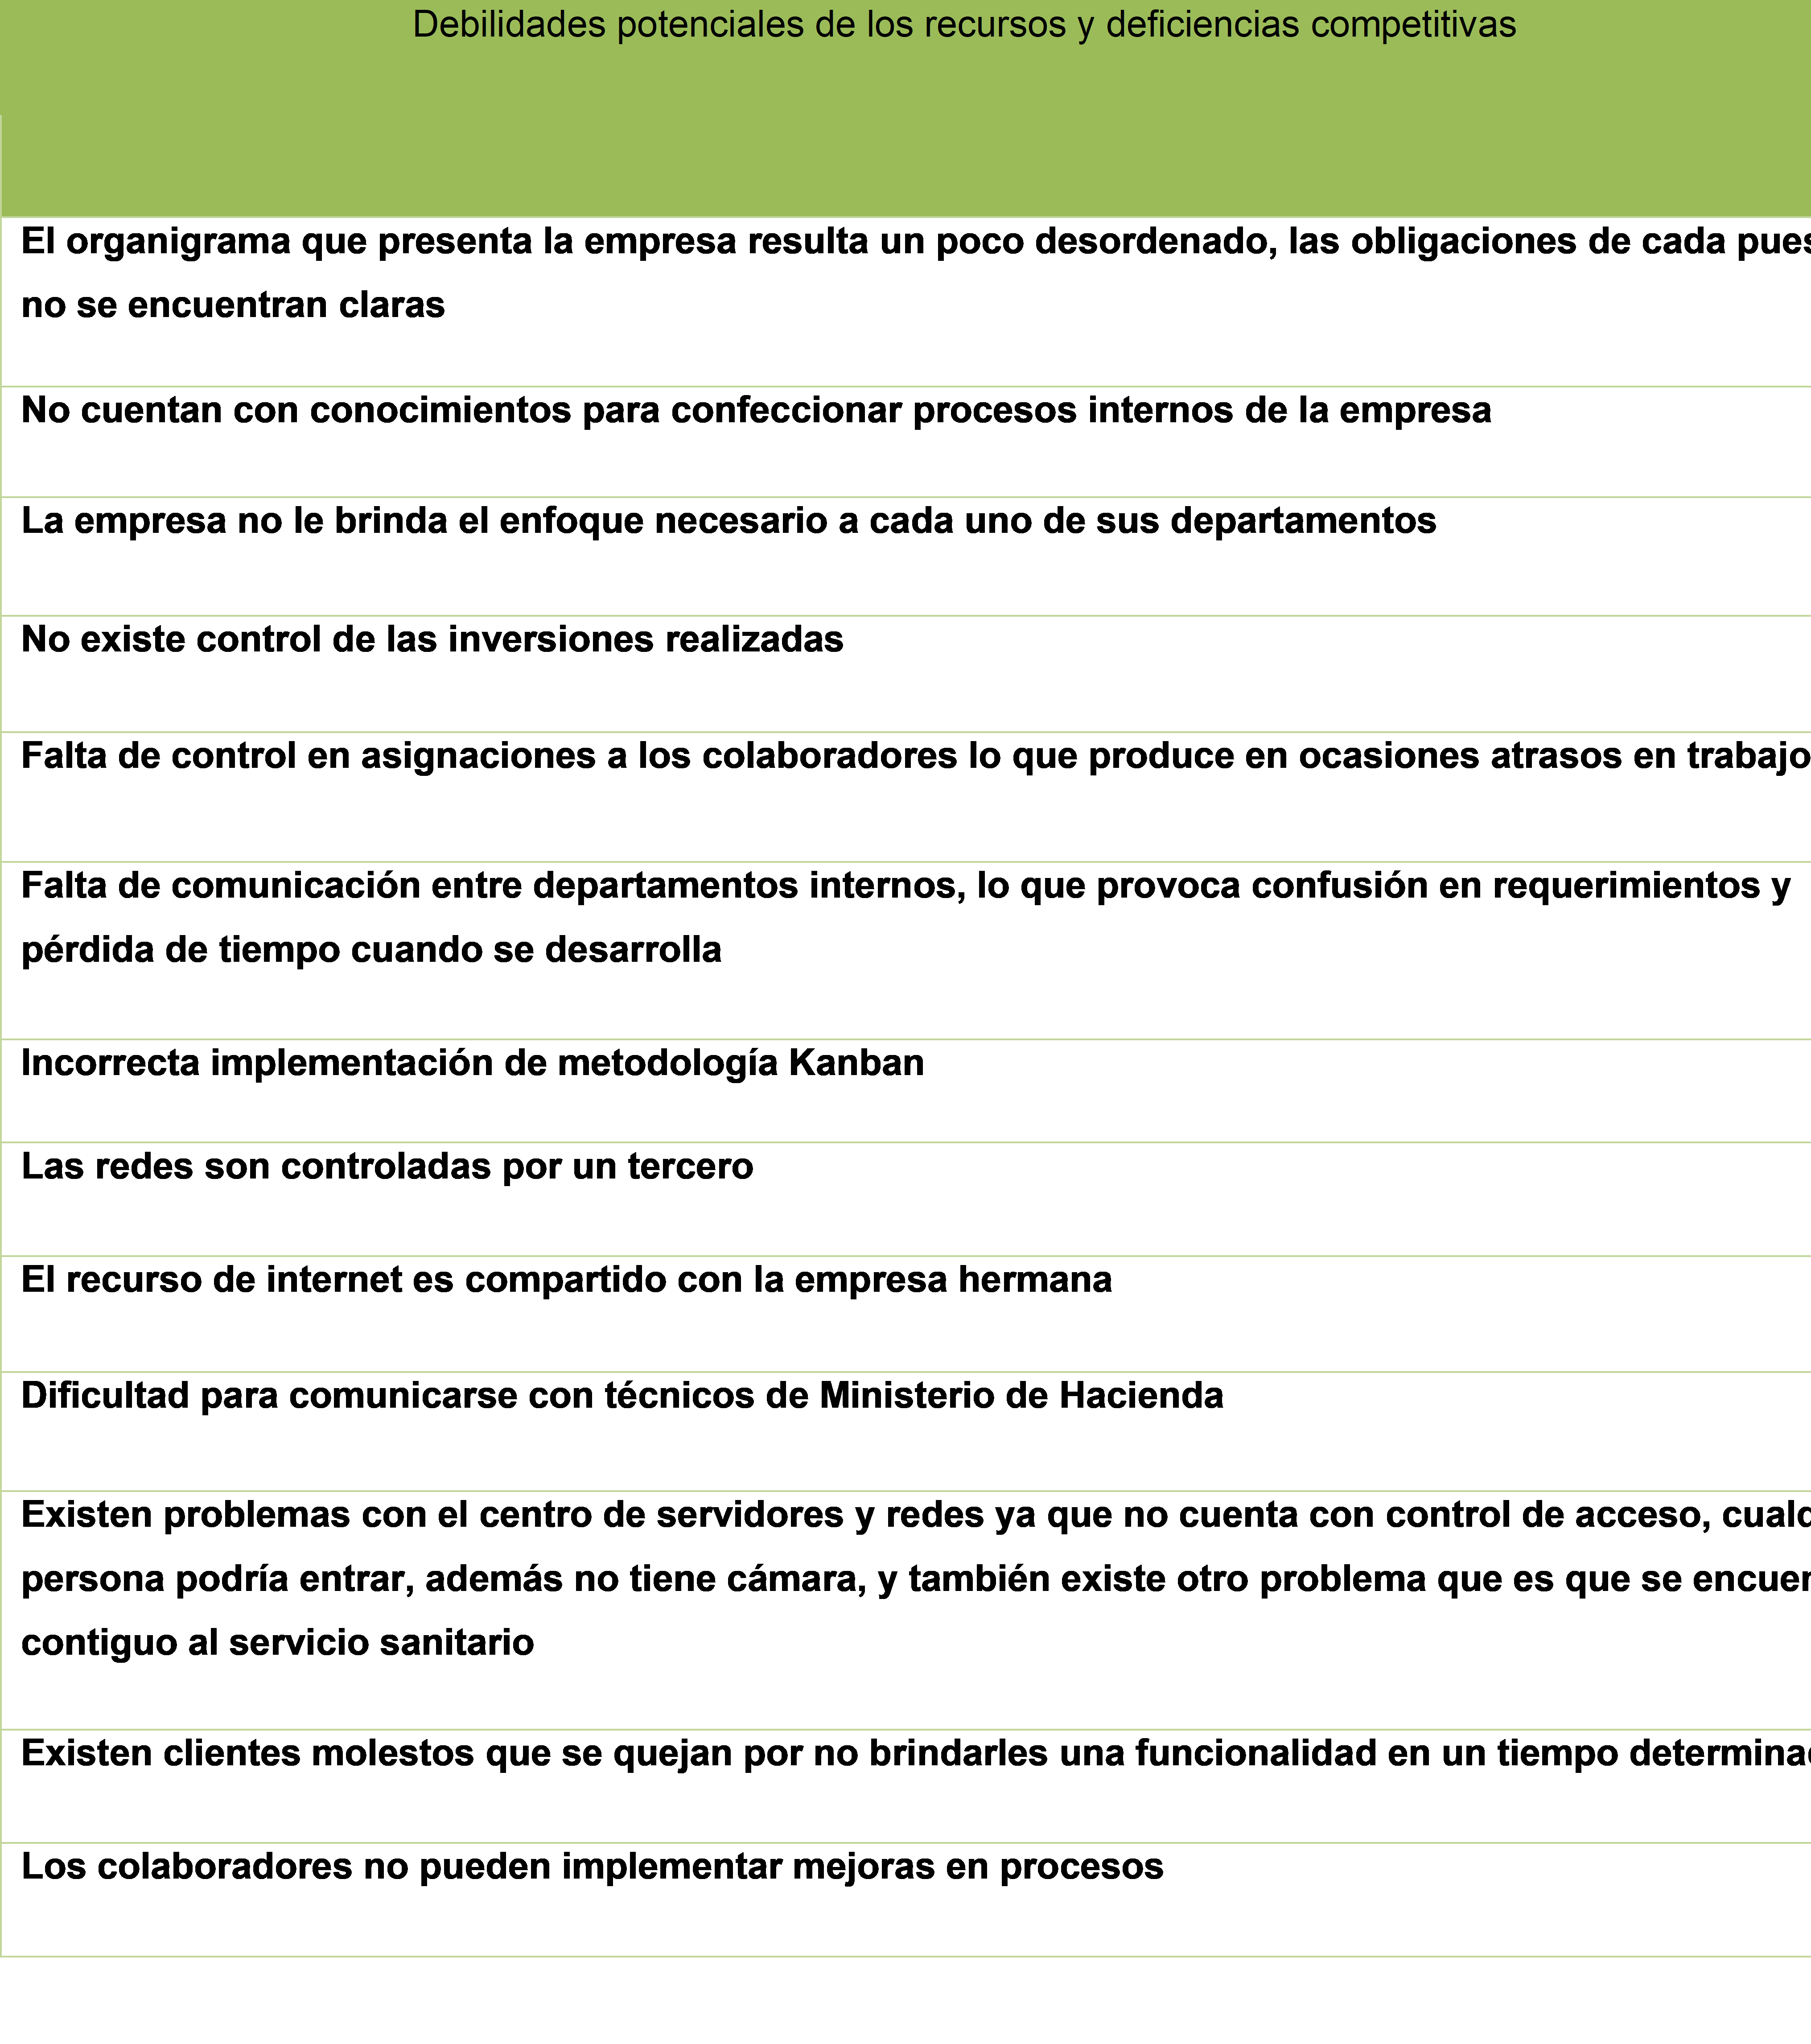
\includegraphics[width=.45\textwidth]{Imagenes/FOFA - Debilidades.png}
        \textbf {Amenazas identificadas}
        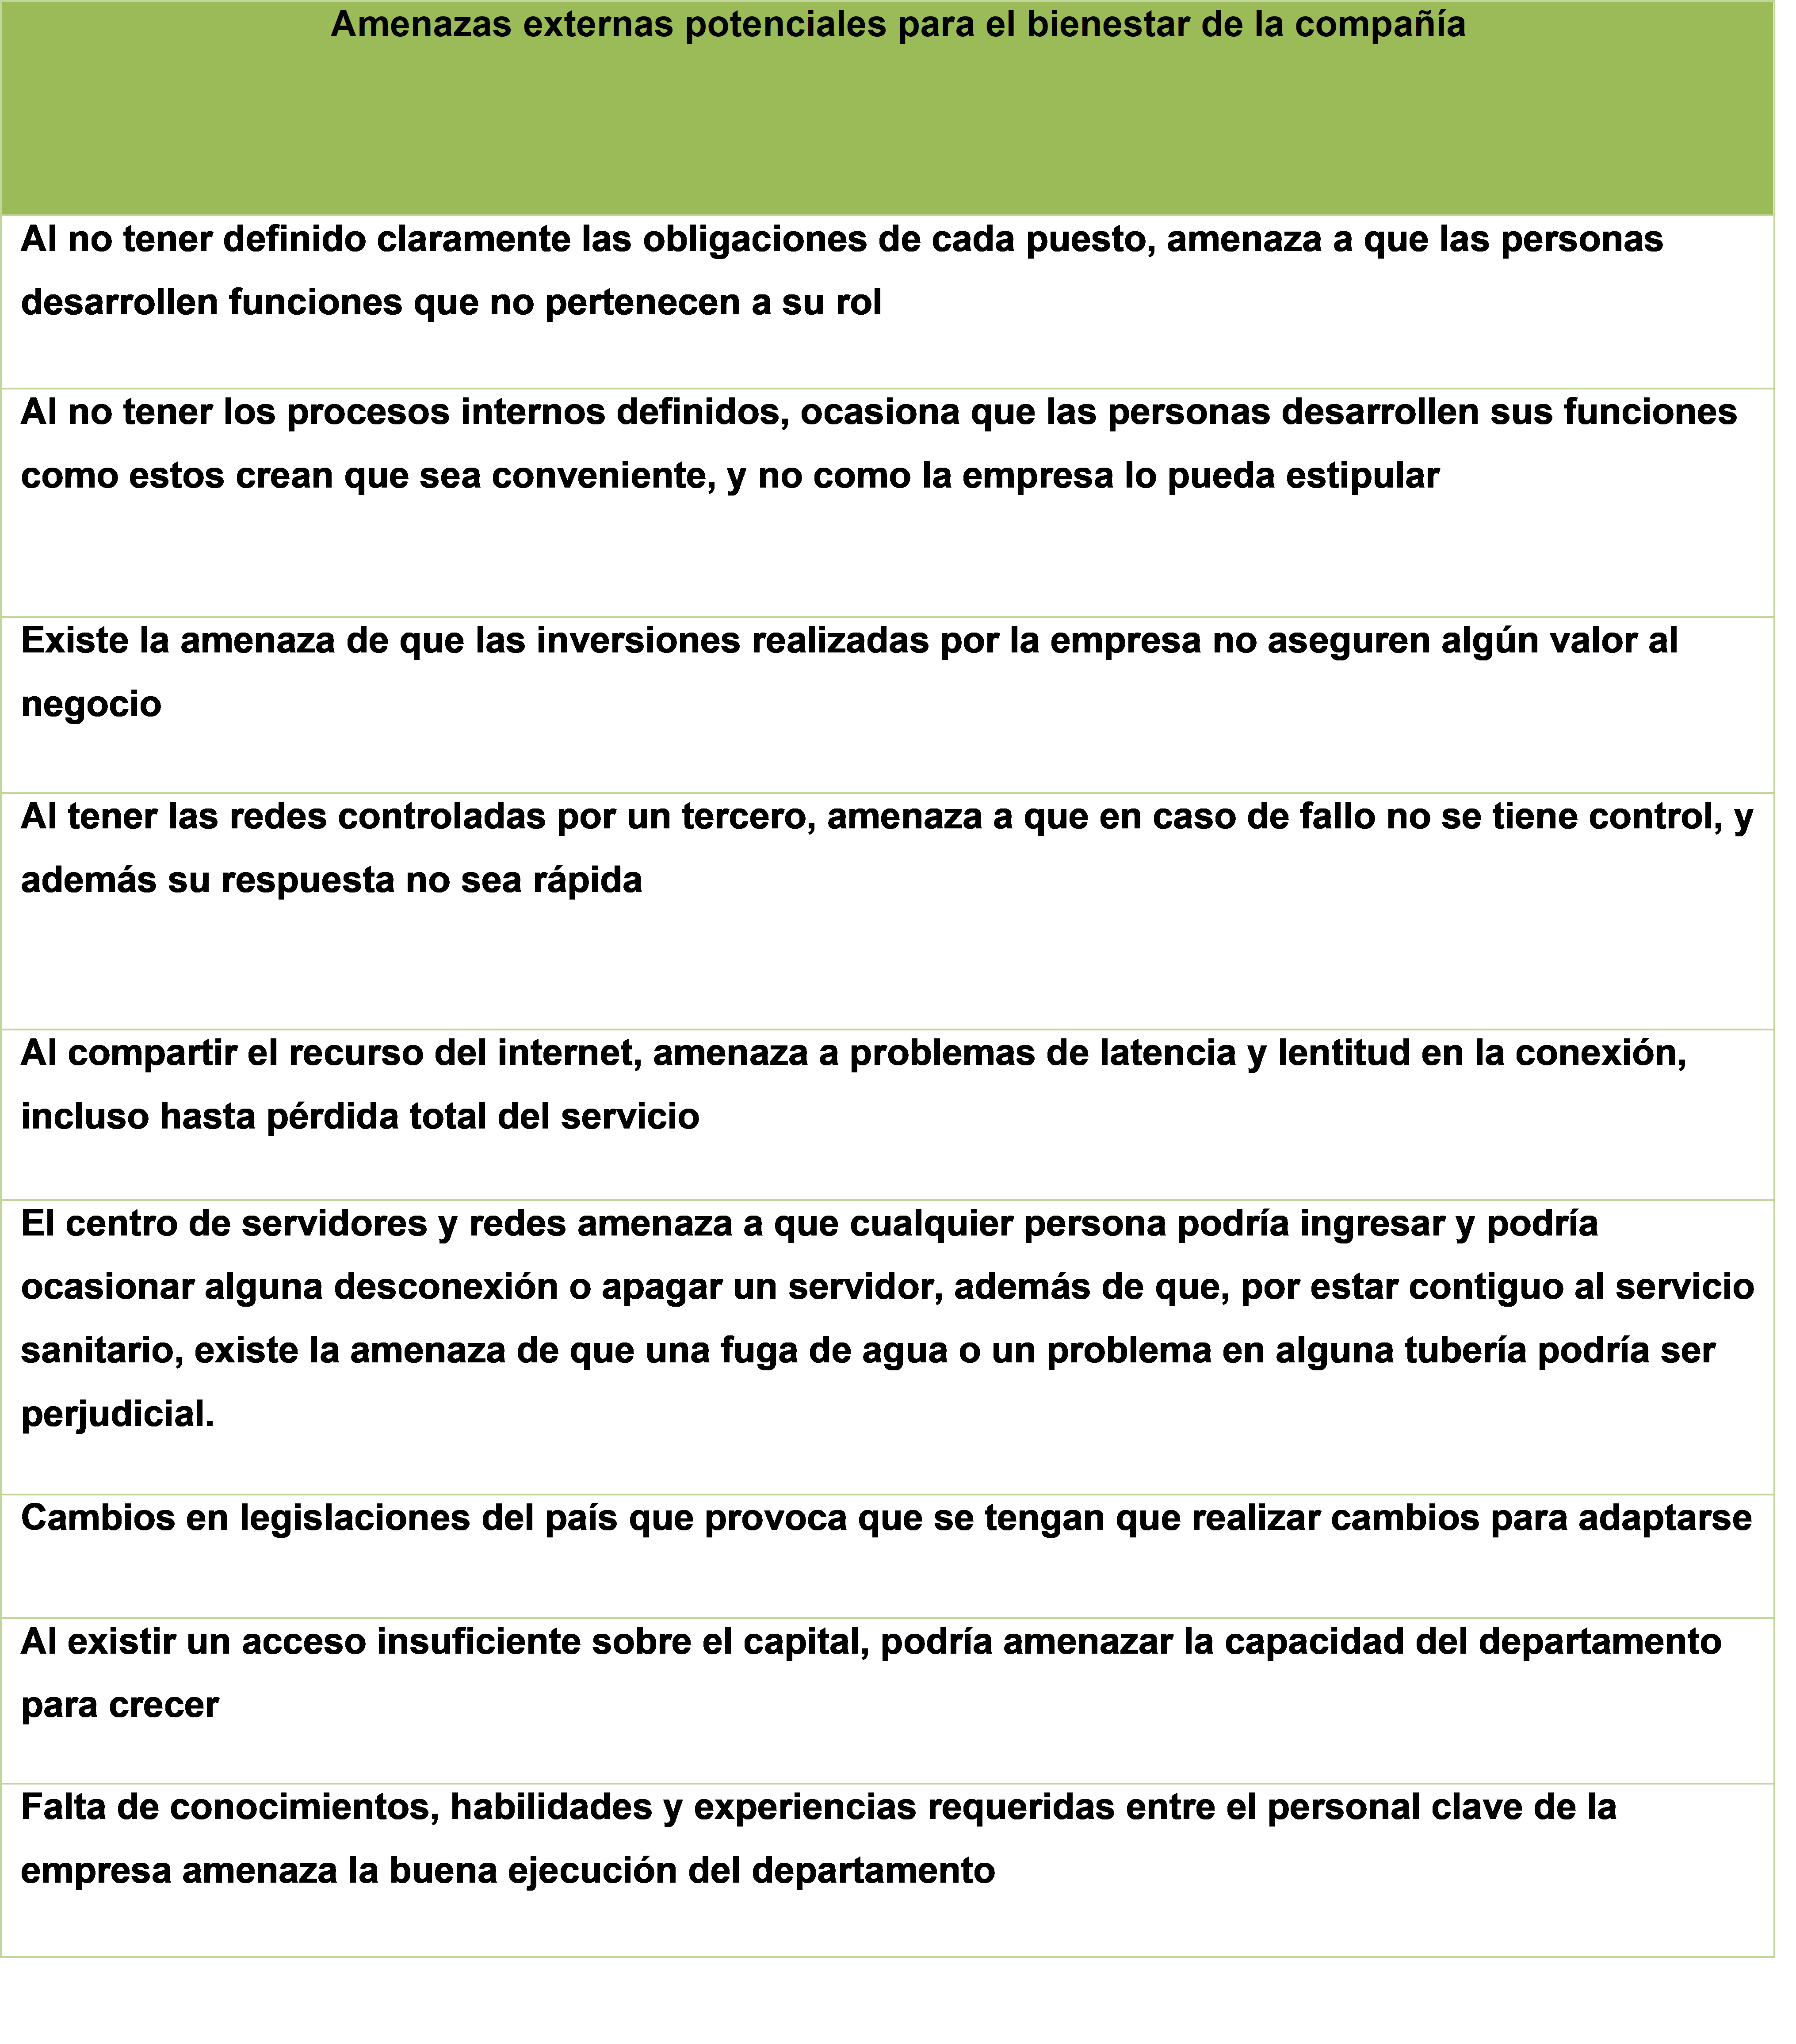
\includegraphics[width=.45\textwidth]{Imagenes/FOFA - Amenazas.png}
    \end{center}

\subsection{Análisis de riesgos}

        \begin{center}
            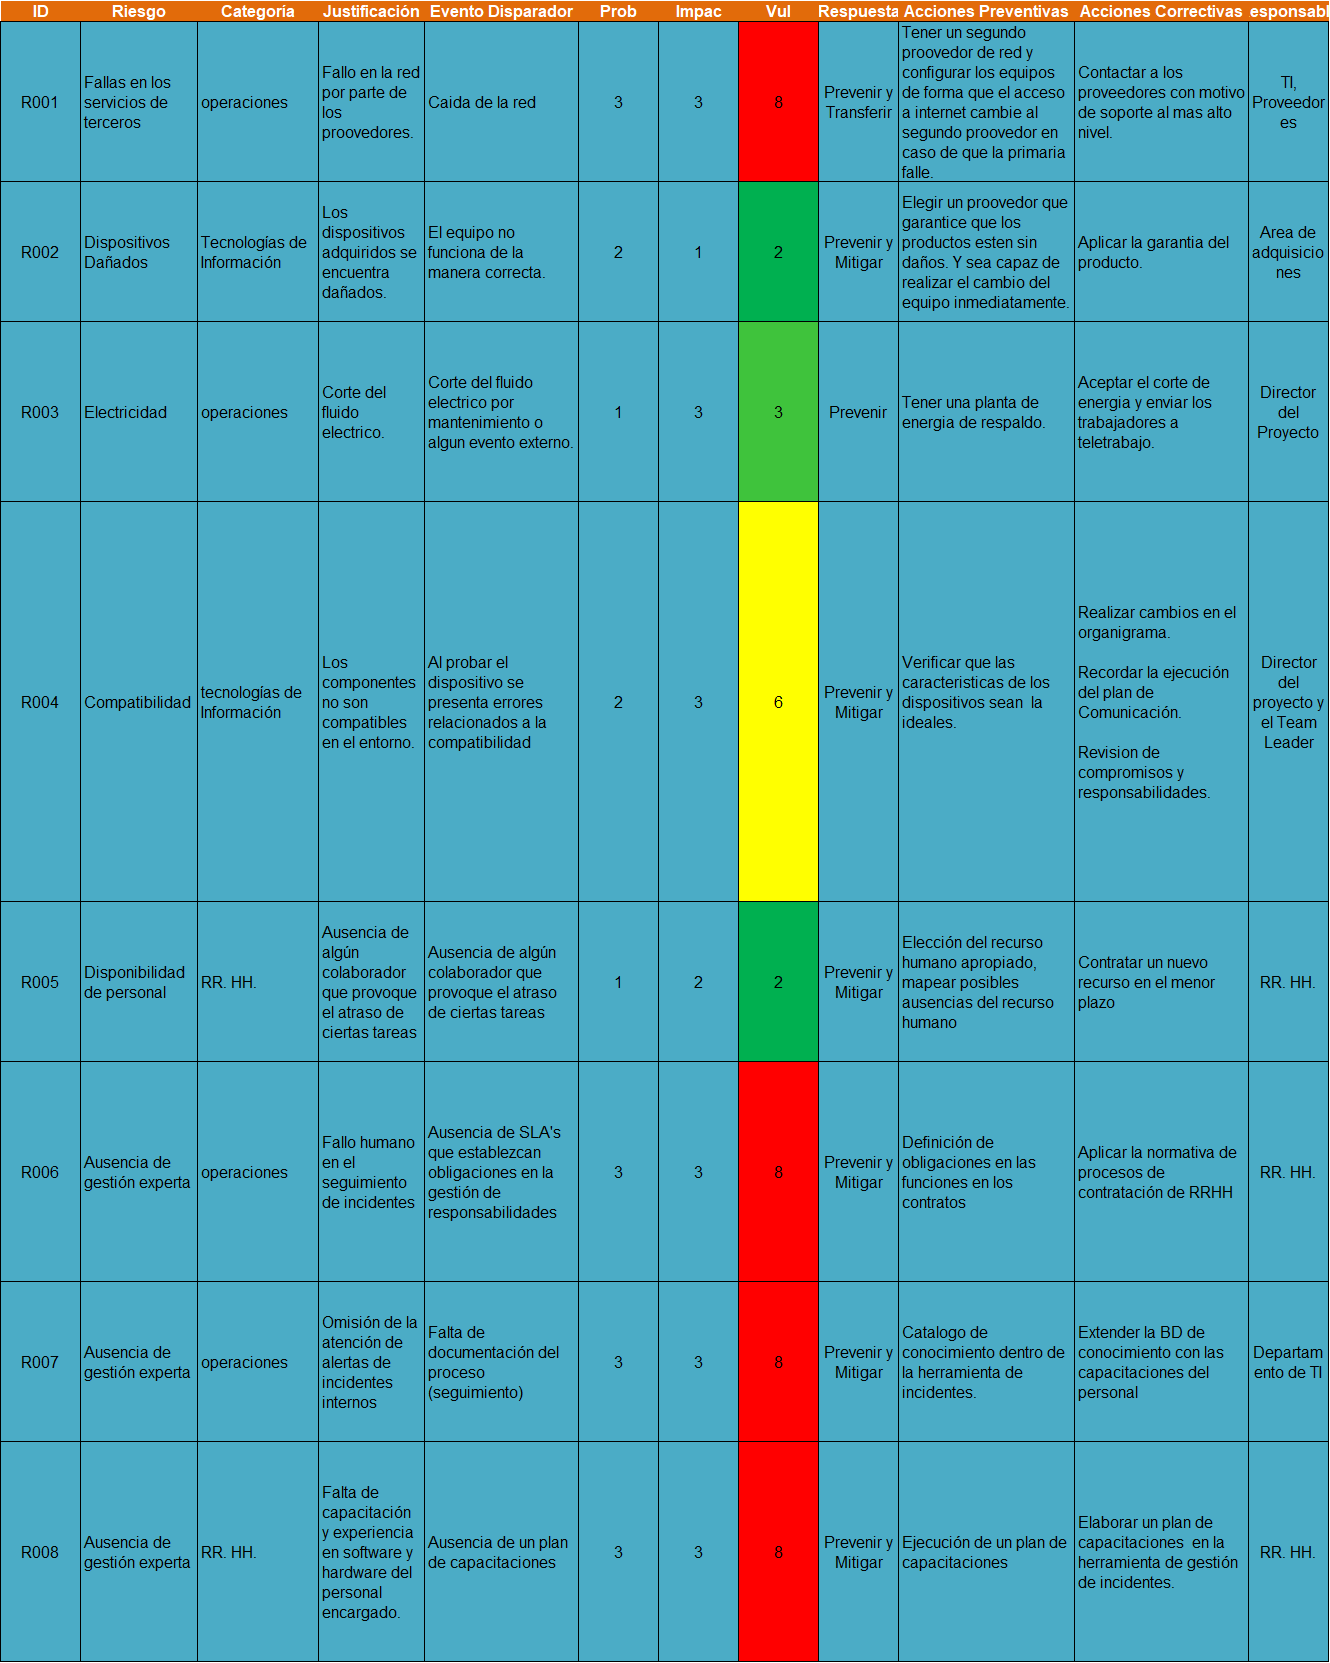
\includegraphics[width=.5\textwidth]{Imagenes/Riesgos.png}
            \textbf {Análisis de Riesgos}
        \end{center}

    \subsection{Análisis del grado de obsolescencia}

        \begin{center}
            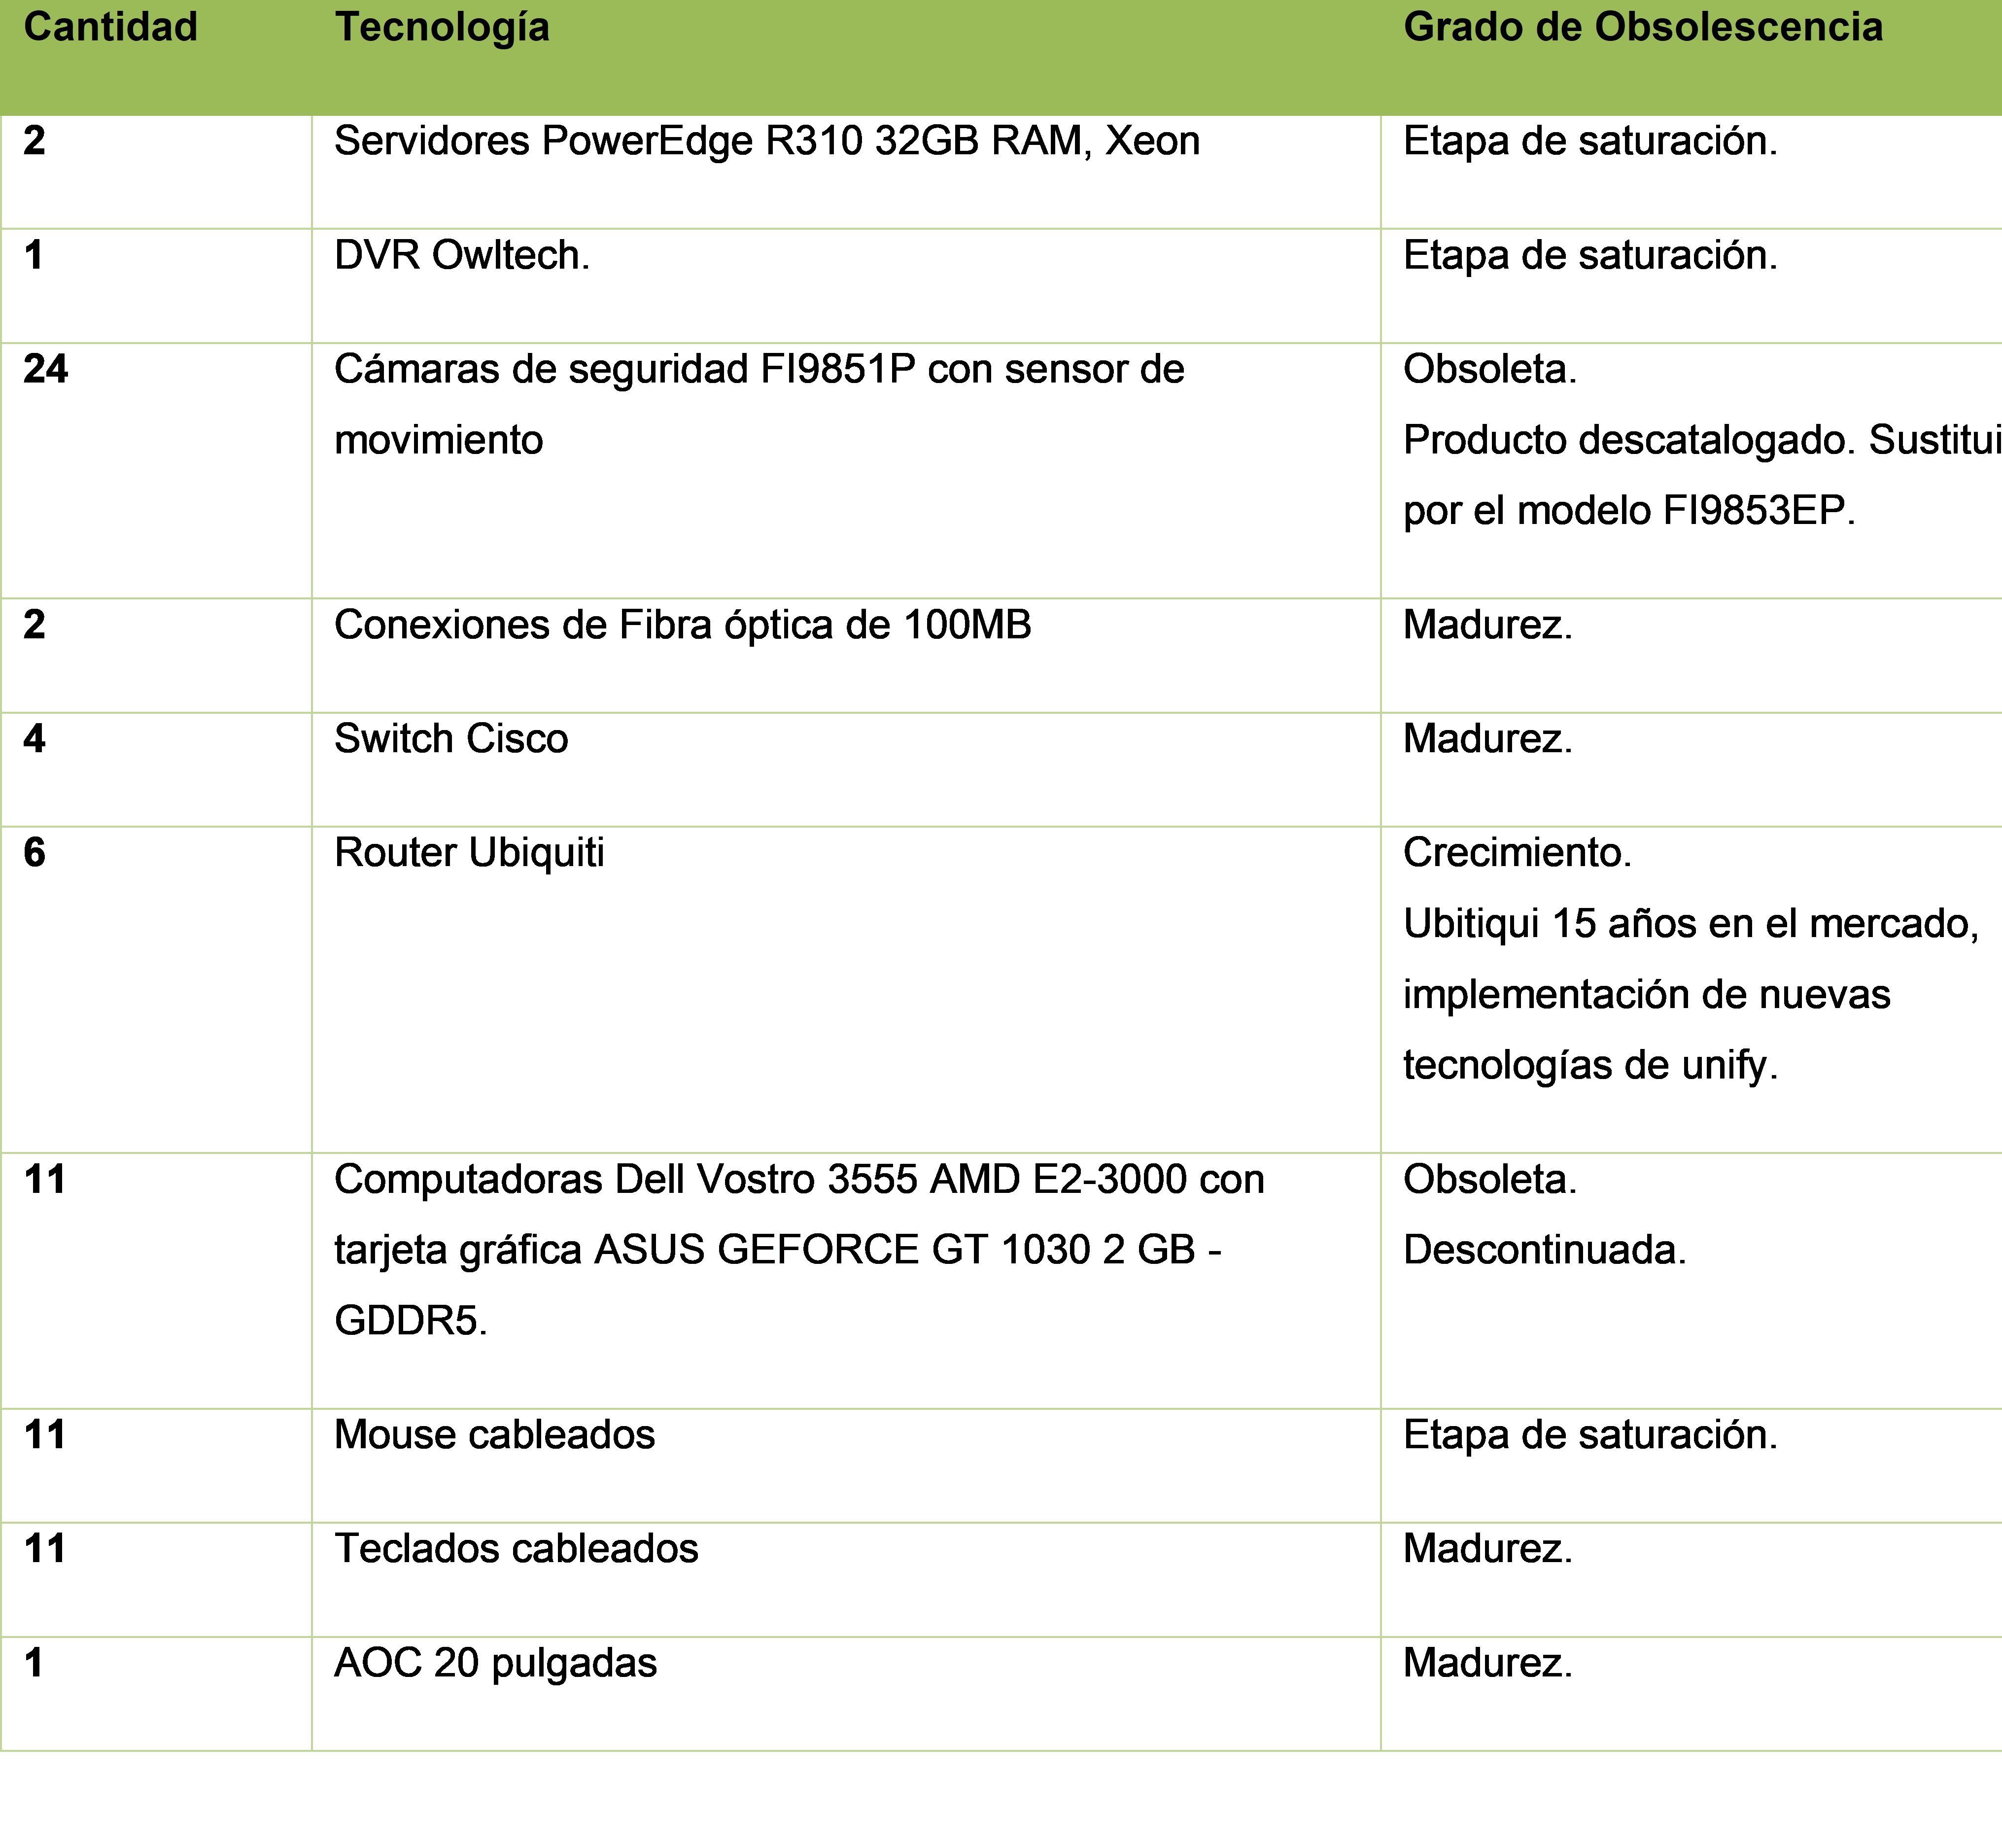
\includegraphics[width=.5\textwidth]{Imagenes/Obsolocencia.png}
            \textbf {Análisis del grado de Obsolescencia}
        \end{center}

\section{Propuesta de la Implementación}
\subsection{Prácticas de gestión de TI a implementar}

Las organizaciones son tan eficientes como lo son sus procesos; las organizaciones que toman conciencia de este hecho se garantizan una buena fluidez de trabajo con un enfoque hacia las metas principales de la entidad y al final la satisfacción del cliente. En este caso la gobernabilidad de TI requiere de algunos cambios y mejoras en cuanto a organización, mejoramiento e implantación de procesos importantes; enseguida se especificarán los procesos actuales y sus mejoras las cuales permitirán una gestión apropiada de los mismos.

    \begin{center}
       \maketitle{(DSS02) Proceso de Gestión de Peticiones e Incidentes de Servicio}
    \end{center}
    \begin{center}
        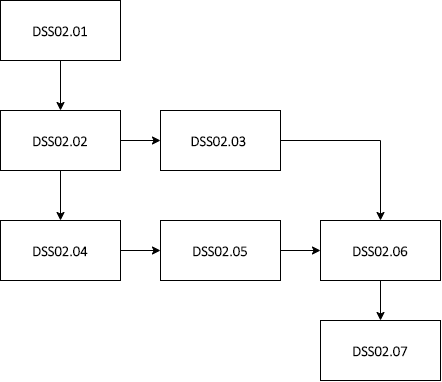
\includegraphics[width=.5\textwidth]{Imagenes/Flujo del proceso catalizador DSS02.png}
        \textbf {Flujo del proceso catalizador DSS02}
    \end{center}
    
\subsection{Estructura organizativa propuesta y matriz RACI asociada.}

\subsubsection{Matriz RACI}

    \begin{center}
        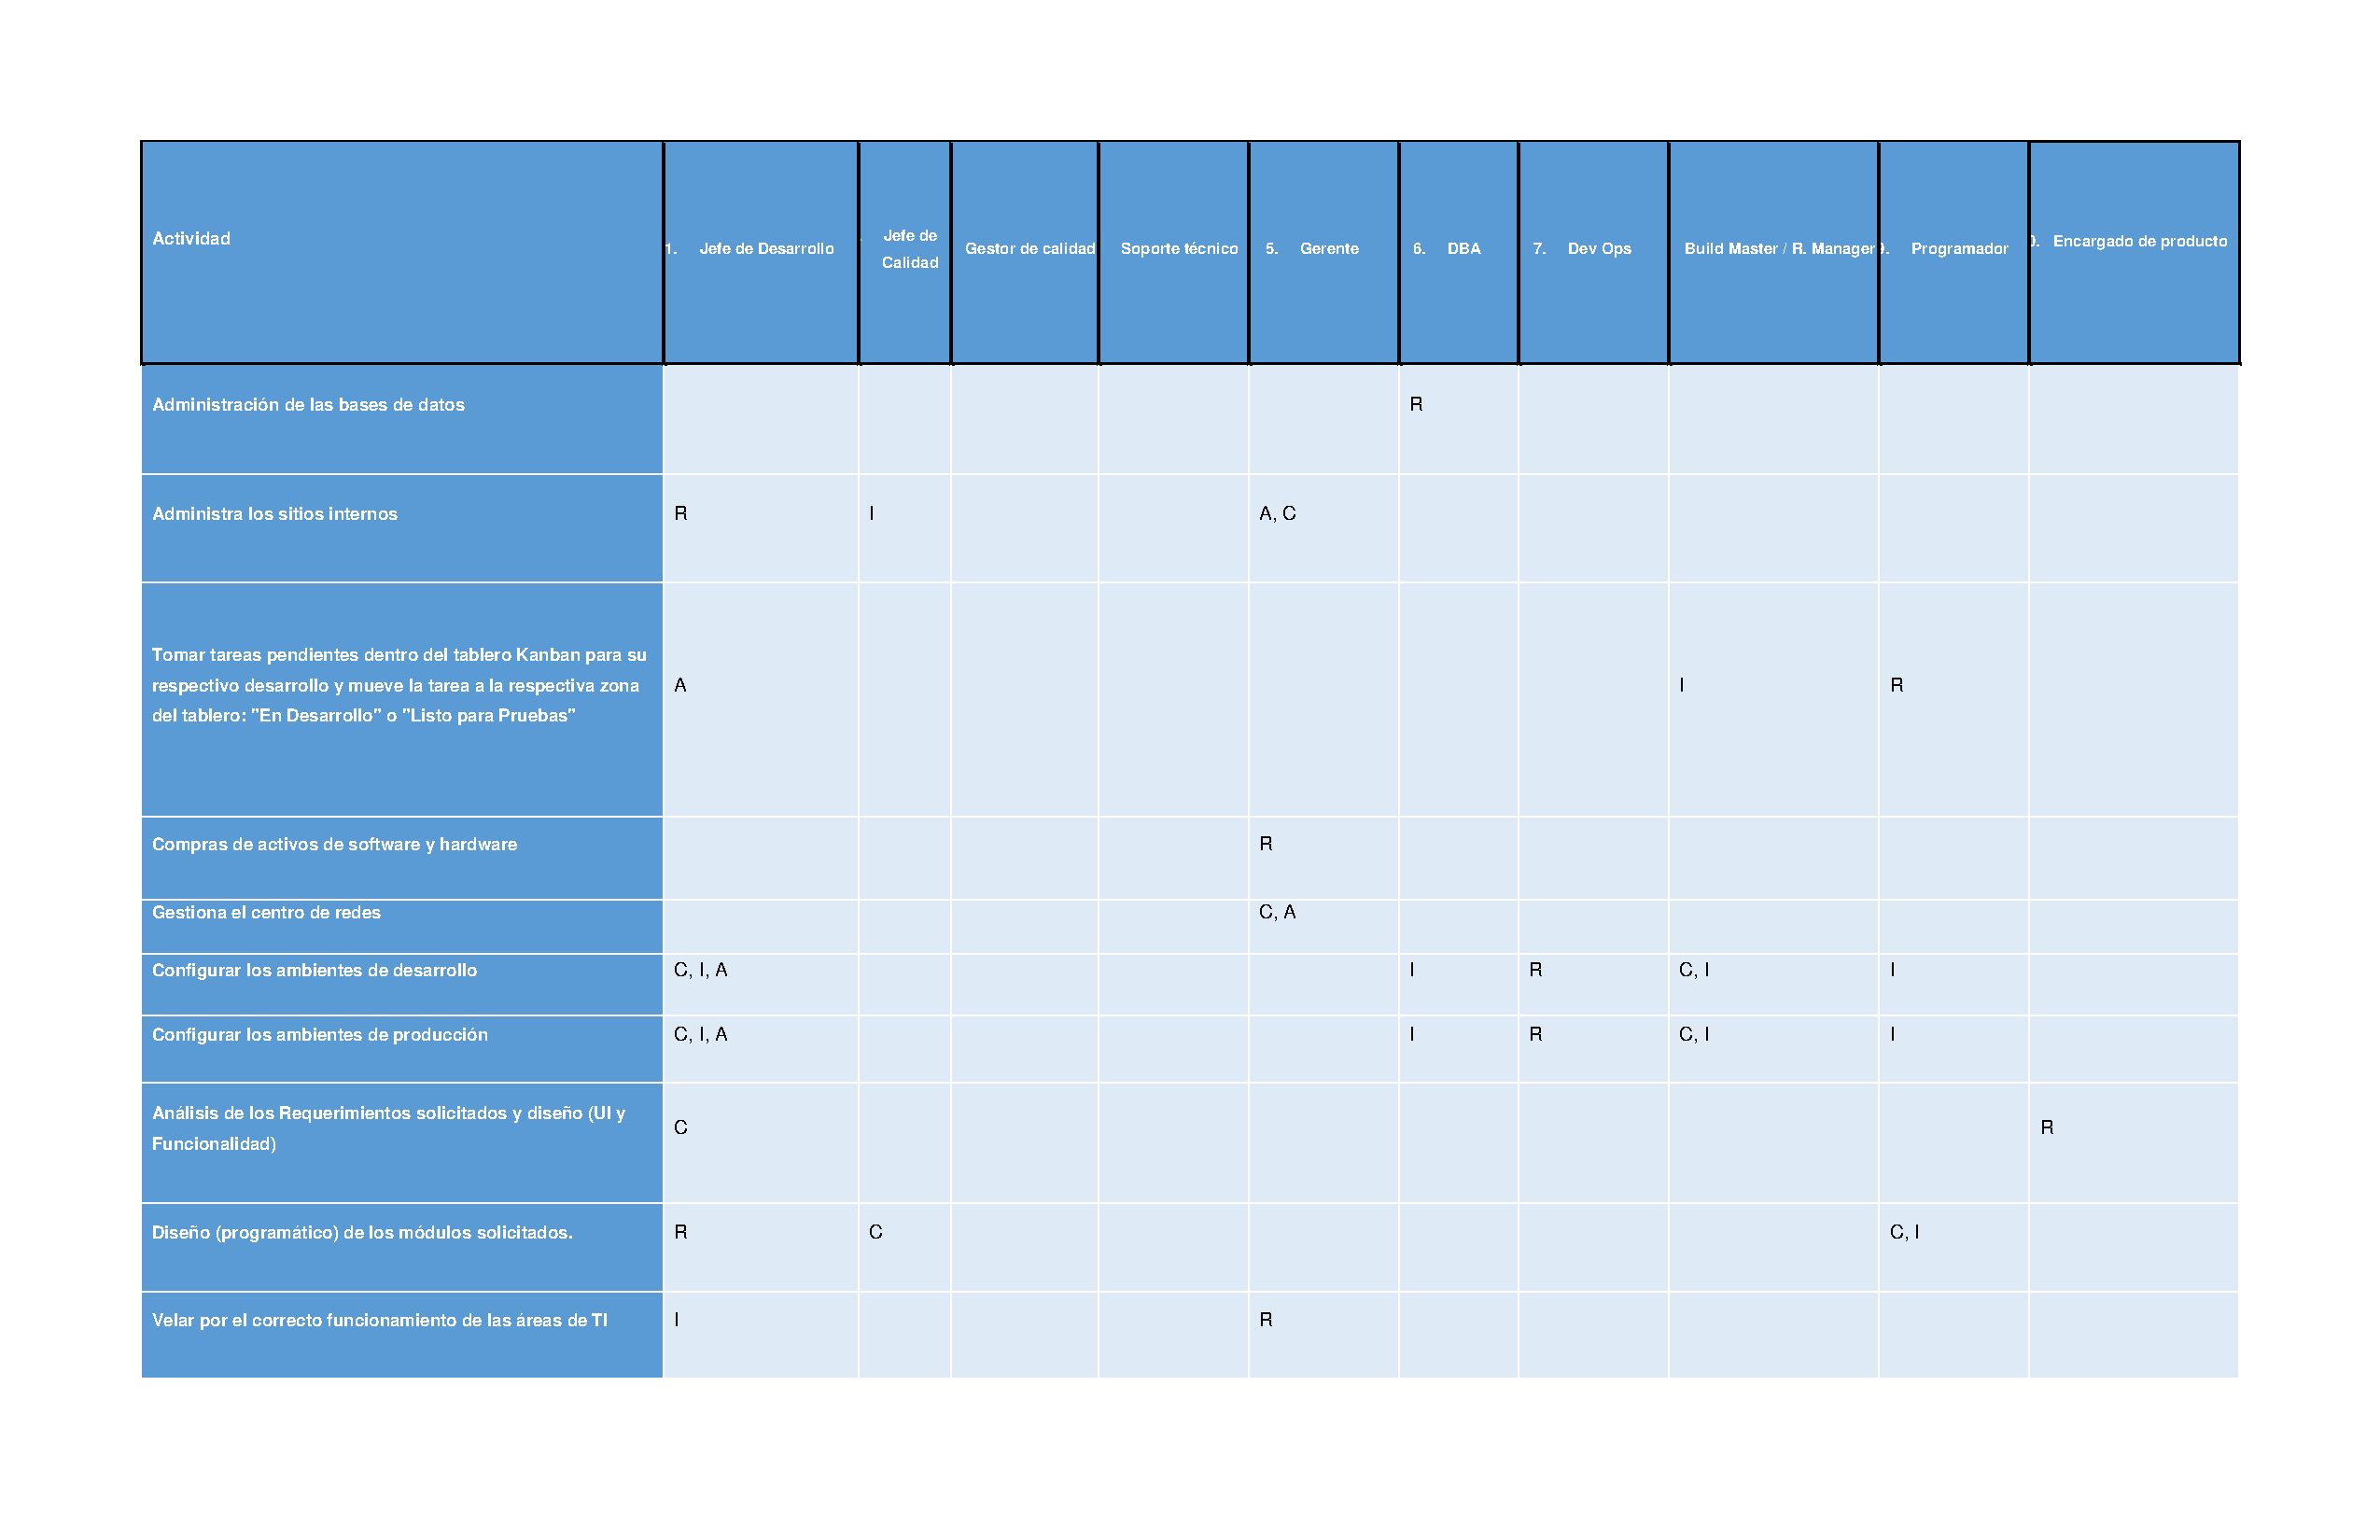
\includegraphics[width=.5\textwidth]{Documentos/Matriz RACI 02.pdf}
    \end{center}

\subsection{Entradas y Salidas}
        \begin{center}
            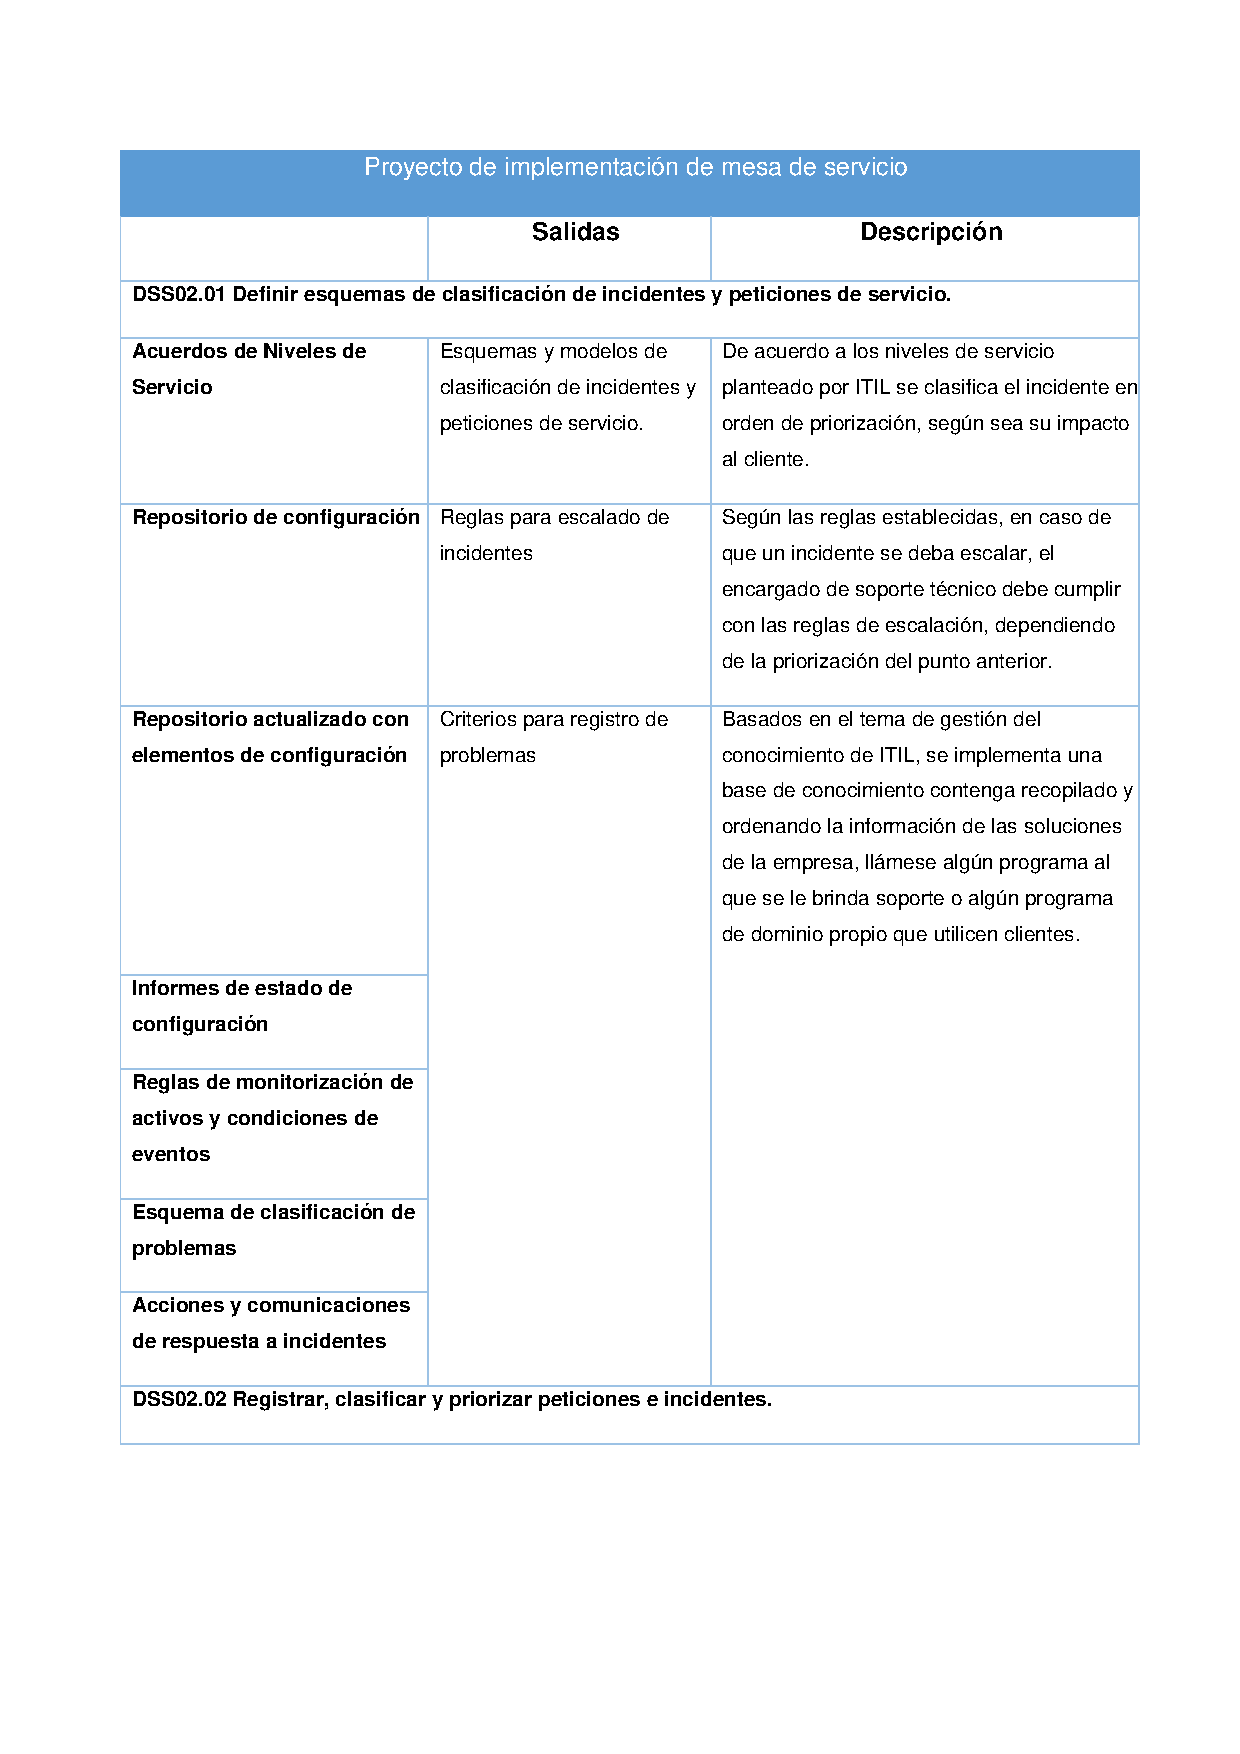
\includegraphics[width=.5\textwidth]{Documentos/Entradas y Salidas.pdf}
            \textbf {Entradas y Salidas de la Implementación}
        \end{center}
        
\subsection{Proyectos asociados a la Implementación de la propuesta}
        \begin{center}
            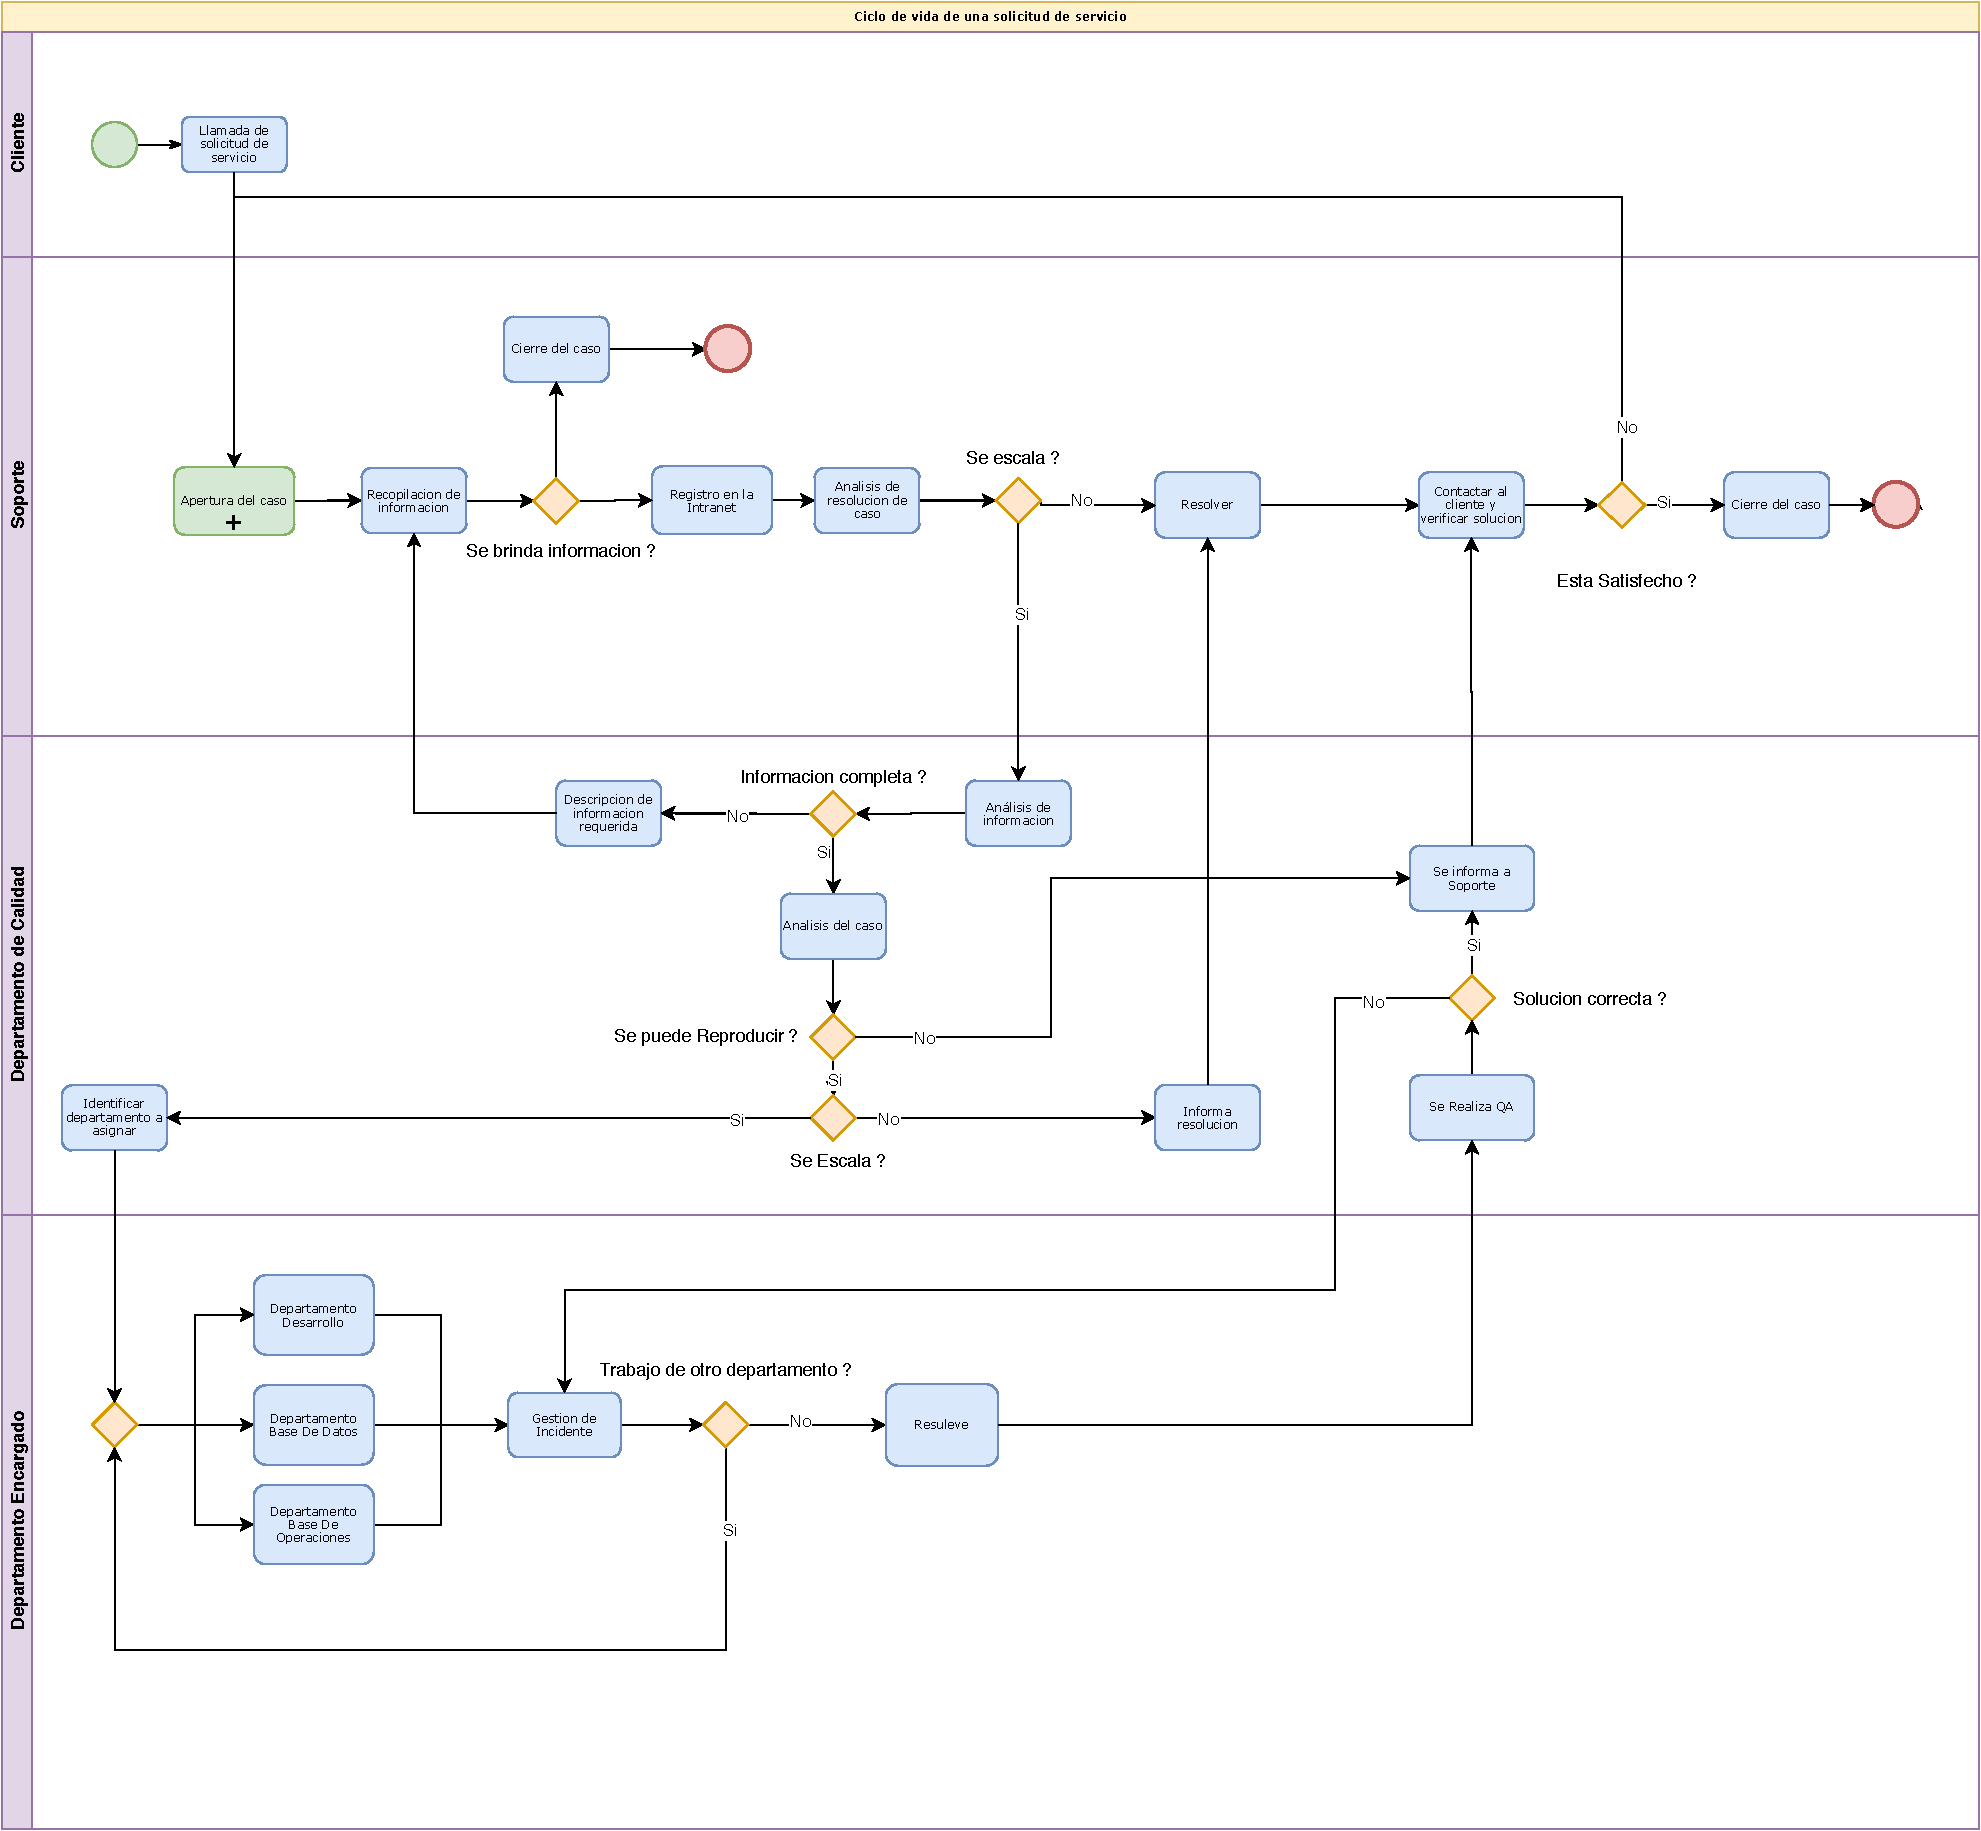
\includegraphics[width=.4\textwidth]{Documentos/Flujo proceso.pdf}\\
            \textbf {Flujo de la propuesta de implementación}
        \end{center}
\newpage
\section{Resultados}

        \begin{itemize}
        \item La definición de todos los recursos que se necesitan como parámetros de entrada para comenzar el proceso
        \item La empresa cuenta con un plan de acción que puede implementar para mejorar los servicios de solicitud de servicio y manejo de incidentes 

        \end{itemize}

\section{Conclusiones}
        \hbox{}
        \begin{itemize}
        \item La utilización del COBIT 5 específicamente en su dominio DSS para definir el proceso de gestión de peticiones de servicio e incidentes de la empresa CentroSoft ayuda a tener un panorama mas claro del paso a paso que se tiene que revisar en el negocio para obtener como resultado un propuesta seria y realista conforme a los estándares de la industria.
        \item Mediante el seguimiento del dominio DSS 04 de COBIT, se ha creado una propuesta que incluye una mejora sobre el proceso de manejo de incidentes y solicitudes de servicio, con el cual la empresa podría tener mejoras en sus operaciones en caso de que se desee implementar todo el plan del proyecto.
        \end{itemize}
        \hbox{}
\section{Recomendaciones}

        \begin{itemize}
        \hbox{}
        \item Para este tipo de implementaciones se recomienda primero siempre definir en términos de alcance del proyecto cual sera el producto final y cuales los procesos atacados desde la perspectiva de mejora de gestión y gobierno de TI, ya que si desde el principio no se mantiene clara la meta, sera muy difícil a lo ultimo aterrizar y concluir el proyecto y su implementación.
        \item 
        \end{itemize}
        \hbox{} 


\begin{thebibliography}{9}
\hbox{}
\bibitem{AXELOS} 
AXELOS (2019)  \textit{ITIL Foundation ITIL 4 Edition}. United Kingdom: TSO (The Stationery Office), part of Williams Lea. \\

\bibitem{Fabregas, J. L} 
Fabregas, J. L. (2009).  \textit{Tecnologías de Información, Gerencia de Servicios. } Caracas: Universidad Católica . [En linea] \url{https://repository.usta.edu.co}\\
\bibitem{Meza, F}

Meza, F (2020, Agosto 06).  \textit{PROPUESTA PARA IMPLEMENTAR ITIL V3 PARA EL SERVICIO DE TELEPRESENCIA.}  [En linea]
\url{https://repository.usta.edu.co/bitstream/handle/11634/2834/Mesadiego2014.pdf?seque}\\

\bibitem{Heikkinen} 
Sanna Heikkinen, A. S. (2013).  \textit{Creating a ITIL-based Software Incident Categorization Model for Measurement: A Case Study. ICSEA, 453.} \\

\bibitem{ISACA} 
ISACA. (2012).\textit{COBIT 5 Procesos Catalizadores} . Illinois: ISACA. \\

\bibitem{García, J} 
García, J., M. A. (2015). \textit{Análisis y propuesta e implementación de las mejores practicas de ITIL.} [En linea] \url{https://dspace.ups.edu.ec/bitstream/123456789/10305/1/UPS-GT001202.pdf} \\

\bibitem{LOZANO F} 
Lozano, F. (2020, Agosto 08) \textit{MODELO PARA LA IMPLEMENTACIÓN DE ITIL EN UNA INSTITUCIÓN UNIVERSITARIA.}  [En linea] \url{https://repository.icesi.edu.co/biblioteca_digital/bitstream/10906/68000/1/modelo_implementacion_universitaria.pdf}
\hbox{}
\end{thebibliography}
\end{document}